\documentclass[pt]{article}  % Sets the font size to 12pt
\usepackage[utf8]{inputenc}
\usepackage{amsmath} % For math formatting
\usepackage{url} % For proper URL formatting
\usepackage{hyperref} % Enables clickable links
\usepackage{tabularx} % Add this in the preamble
\usepackage{float} % Add this to the preamble
\usepackage{geometry} % Adjust page layout
\usepackage{graphicx}
\usepackage{multirow} % For multi-row cells
\usepackage{subcaption} % For subfigures
\usepackage{float}
\usepackage{booktabs}
\usepackage[utf8]{inputenc}

\hypersetup{
    colorlinks=true,       % Enables colored links instead of boxes
    linkcolor=blue,        % Sets link text color to blue
    filecolor=blue,        % Sets file link color
    urlcolor=blue,         % Sets URL link color
    citecolor=blue,        % Sets citation link color
    linkbordercolor={0 0 0}, % Removes red borders around links
    pdfborder={0 0 0}      % Removes borders in the PDF view
}
\geometry{a4paper, margin=1in}
\usepackage{caption}
\usepackage{cite} % For references
\title{ Predictive Analysis of Political Partisanship with Machine Learning: A Comparative Study of Online and Offline Arenas}
\date{}
\begin{document}

\maketitle

% Abstract
\begin{abstract}
\large Political partisanship is a growing global concern, affecting societal stability and governance. The growing ideological divides across societies underscore the urgent need to understand the factors of partisanship. This study leverages machine learning techniques to predict political partisanship by analyzing survey data collected from three diverse countries: the United Kingdom, Malaysia, and Pakistan. The dataset incorporates factors such as voluntary online and offline participation, social media utilization for political purposes, offering a comprehensive view of factors driving towards political partisanship. By training predictive models on this dataset, we identify key determinants of partisan alignment and examine their varying significance across sociopolitical settings. This study provides actionable insights for policymakers, enabling the development of tailored strategies to mitigate polarization and foster political cohesion. The best-performing model achieved an accuracy of 87\%, demonstrating its efficacy in identifying key predictors of partisan alignment. Later, the Explainable AI was applied to interpret the model's predictions, revealing the relative importance of features like offline participation and social media usage. The study also includes cross-country validation by training the model on one specific country’s data and testing it on the other two, which provides a broader understanding of partisanship in varying sociopolitical contexts and highlights the versatility of political behavior patterns across different nations. 
\end{abstract}

\section{Introduction}
\large Political researchers and theorists have long been devoted to understand the complexities of governance, power, and public sentiment. Figures like Alexis de Tocqueville, whose seminal work 'Democracy in America' remains a foundation of political analysis, or Max Weber, the architect of modern political sociology, spent their lives to unravel the dynamics of political systems and public behavior. Now, it is our turn to explore the interplay between online and offline platforms on political partisanship through predictive modeling.

The rise in partisan politics has become a prominent phenomenon across the world, manifesting in various forms and intensities in both developed and developing countries. Recent research indicates that political polarization is not confined to the United States only, but is increasingly evident in nations with diverse political landscapes\cite{ref1}. Developed country such as The UK and developing countries like Malaysia and Pakistan has faced detrimental political upheaval due to partisan politics. In the UK, for example, partisan affective polarization has significantly increased particularly in the last decade. This growing polarization is largely driven by partisan identity rather than ideological differences\cite{ref2}. Also the unprecedented increase in political polarization in Pakistan, as evidenced by the 2022 ouster of key political figures and the subsequent societal divisions\cite{ref3}, increases the need for examination of the underlying factors driving partisanship. Thus, it is essential to know the key factors that coerces political partisanship for nurturing constructive dialogue and developing effective policies.

In this research, we aim to explore the levels of partisanship in the three countries-UK, Malaysia and Pakistan. We analyze key variables such as \textbf{social media utilization}, \textbf{online social capital}, \textbf{voluntary online participation}, \textbf{voluntary offline participation}, and \textbf{political trust} as critical factors influencing political behavior and partisanship. By employing machine learning models on the dataset derived from a survey containing data from these three regions. The survey has been constructed based on the \textbf{Motive-Incentive-Activation-Behavior (MIAB)} model\cite{ref4}. The MIAB framework highlights how crucial it is to connect motivation, incentives, and activation to encourage meaningful participation. Using insights from the survey, this study aims to predict political partisanship by exploring how factors like social media engagement, voluntary political participation, or trust in governance shape individuals’ political affiliations. Fig.~\ref{fig:figure1} shows the framework:\vspace{0.5cm}

% First Figure
\begin{figure}[h]
    \centering
    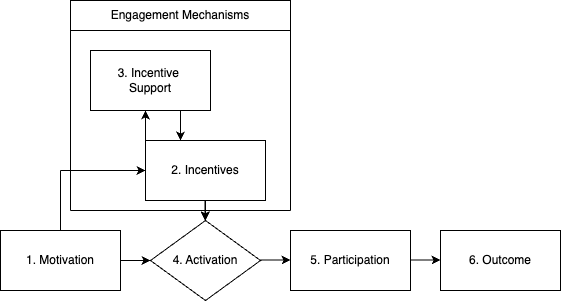
\includegraphics[width=13cm, height=7cm]{Project445/MIAB.png} % Replace with your image file
    \caption{\textbf{The Motive-Incentive-Activation-Behavior Model}\cite{ref5}.}
    \label{fig:figure1}
\end{figure}

This study aims to integrate the theoretical framework with machine learning approach to explore individual's behavioral insights in political partisanship. To handle complex data patterns and improve predictive accuracy, ten different algorithms including four ensemble learning classifiers and one neural network. After selected the best performing model, explainable AI (LIME) is used on that to interpret the model's action. Findings of the XAI suggests, while online participation and engagement play a significant role in shaping political preferences, offline activities remain a crucial factor in influencing political alignment. The approach also involves a cross-country model, where the model is trained using data from one specific country and then tested separately on data from two other countries. Lastly, some edge cases, such as uniform responses to all the questionnaire of the survey was manually input to test the model's capability in handling unrealistic environment. 

% Related Work
\section{Literature Review}
Numerous studies regarding political polarization has been conducted. Existing studies often focus on specific demographics or regions, leaving a gap in understanding partisanship across diverse contexts. Research on developing nations, where cultural and economic factors uniquely shape political behavior, remains limited. Our work addresses this gap by analyzing data from several locations to explore cross-national variations in partisanship. Very few studies have integrated the MIAB model with machine learning to analyse individual's political behavior. Emese, Angya and Zita Fellner \cite{ref6} finds that online political participation positively influences offline political activities. Using Bayesian updating, the paper synthesizes studies from 2009–2019, showing social media effectively mobilizes offline engagement despite methodological challenges like self-reported data and demographic biases. Yahhuei Hong1, Trisha T. C. Lin \cite{ref7} examines how family, peers, and media influence Singaporean youth's political participation using survey data that shows family and peer discussions boost both online and offline engagement, while online news exposure primarily supports online participation. Prasad Hajare et al \cite{ref8} develops a machine learning pipeline to analyze political bias in social media using the U.S. congressional speeches for labeling. It predicts bias in posts with 70.5\% accuracy and forecasts bias shifts with 85\% accuracy, leveraging features from text and conversation cascades. Veronica Cagle \cite{ref15} uses a neural network to classify Reddit comments as polarized or not, achieving 75-80\% accuracy. The study finds no overall polarization increase but detects trends in specific subreddits tied to political events. Sadia Kamal \cite{ref10} develops heuristic labeling methods and machine learning models to predict the political orientation of social media posts, achieving up to 99\% accuracy with BERT on Gab data. The research highlights scalable approaches to analyze online polarization. Table~\ref{tab:table1} reviews key contributions and highlights gaps in some of the existing literature:


\begin{table}[H] % Use [H] to enforce the table's exact location
    \centering
    \begin{tabularx}{\textwidth}{|X|X|X|}
        \hline
        \textbf{Title} & \textbf{Advantages} & \textbf{Limitations} \\ \hline How are Online and Offline Political Activities Connected? A Comparison of Studies\cite{ref6} 
        & Synthesizes evidence across diverse research designs using innovative Bayesian updating methodology
        & Uses self-reported data, lacks machine learning approach \\ \hline
        The Impacts of Political Socialization on People’s Online and Offline Political Participation—Taking the Youth of Singapore as an Example\cite{ref7} 
        & Effectively identifies the influence of political socialization on both online and offline political participation 
        & Limited to a specific geographic and cultural context (Singapore) \\ \hline
        A Machine Learning Pipeline to Examine Political Bias with Congressional Speeches\cite{ref8} 
        & Introduces a novel machine learning pipeline that labels political bias in social media posts 
        & Dataset focused on specific platforms, few algorithms are applied \\ \hline
        The slacktivism crossroad: causal relationships between online and offline political participation\cite{ref9}
        & Provides a comprehensive analysis demonstrating the persistent positive effects of online political participation on offline engagement 
        & Limited diversity in the dataset, focusing on Spanish citizens aged 16–45, lacks machine learning approach \\ \hline


        Using Machine Learning to Measure Political Polarization on Social Media\cite{ref15}
        & Applies natural language processing to measure political polarization, leveraging user-generated content for a novel analysis. 
        & Focuses on specific platform, lacks explainable AI. Primarily evaluated by accuracy only.  \\ \hline
        

         Modeling Political Orientation of Social Media Posts: 
         An Extended Analysis\cite{ref10} 
        & Novel approach to political orientation prediction of social media posts through heuristic labeling 
        & Confined to textual data, omitting multi-modal social media content, lacks explainable AI \\ \hline

    \end{tabularx}
    \caption{\textbf{A comparative analysis of related works on flood evacuation systems.}}
    \label{tab:table1}
\end{table}


% Methodology
\section{Methodology}
The dataset underwent data pre-processing and visualization to explore relationships and derive insights. The data was split by standard protocol. Feature selection was applied to identify key predictors, and machine learning classifiers were optimized through hyperparameter tuning. The best-performing model was evaluated, and Explainable AI techniques were employed to interpret its predictions and uncover the most significant factors driving political partisanship. Fig.~\ref{fig:figure2} illustrates the methodology workflow :

\begin{figure}[H]
    \centering
    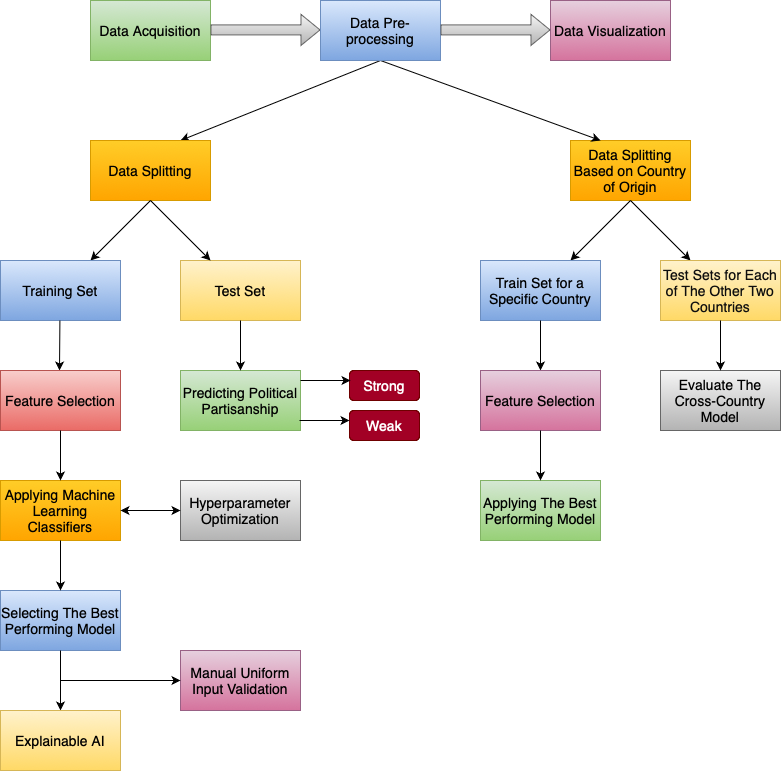
\includegraphics[width=14cm, height=14cm]{Project445/Methodogy.png} % Ensure this path is correct
    \caption{\textbf{The Methodology of the study.}}
    \label{fig:figure2} 
\end{figure}


\subsection{\textbf{Data Acquisition }}The survey used to create the dataset was obtained from the study conducted by\cite{ref4}, wherein 472 people from different regions actively participated. The distribution of the questionnaires was spread through the utilization of Google forms targeting voters who also engaged with social media. The respondents were asked to use a 5-point Likert-scale to express their agreement with 46 statements categorized by six kinds, such as social media utilization, online social capital, voluntary online and offline political participation, ranging from 1 to 5, where 1 defined “Strongly Disagree” and 5 denoted “Strongly Agree’. In contrast, items linked with partisanship were assessed using a scale ranging from 1 to 5, where 1 indicates “Weak” and 5 indicates “Extremely Strong”. Alongside their opinions on the statements, some personal information were also recorded, such as country of origin, religion, gender, age, marital status, education level, employment, political ideology.

\subsection{Data Visualization}

\subsubsection{Respondents Distribution}

Fig.~\ref{fig:gender-Distribution} shows the gender distribution of respondents that defines a significant majority identifying as male (61.9\%), while a smaller proportion identifies as female (38.1\%). This highlights a noticeable male dominance among the survey participants.

Fig.~\ref{fig:Age_Distribution} below shows the age distribution of respondents, with the largest group being 18-28 years old (37.3\%), followed by 29-39 years old (25.2\%). Smaller groups
include 40-50 years old (20.6\%), 51-60 years old (10.4\%), and Above 60 years old (6.1\%),
while 0.4\% preferred not to answer.

Fig.~\ref{fig:religion-Distribution} demonstrates the religion distribution of the respondents is varied, with Islam as the dominant category (54.9\%). Christianity accounts for 14.0\% of the responses, followed by Buddhism and “Prefer not to answer,” both at 8.7\%. Other religions like Hinduism (2.8\%), Atheism (6.8\%), and Judaism (0.4\%) also have minimal representation.




\begin{figure}[H]
    \centering
    \begin{minipage}[b]{0.3\textwidth} % Adjust width as needed
        \centering
        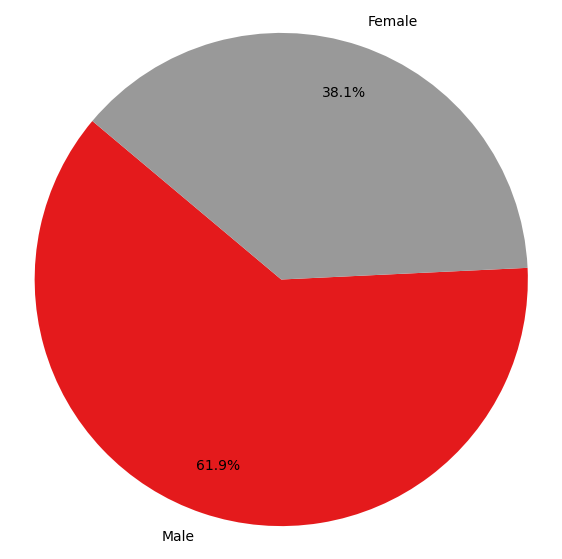
\includegraphics[width=4.7cm, height=4.8cm]{gender-Distribution.png} % Fixed width
        \caption{Gender} % Add your caption here
        \label{fig:gender-Distribution} % Add a label for referencing
    \end{minipage}
    \hfill
    \hspace*{-1cm}
    \begin{minipage}[b]{0.3\textwidth} % Adjust width as needed
        \centering
        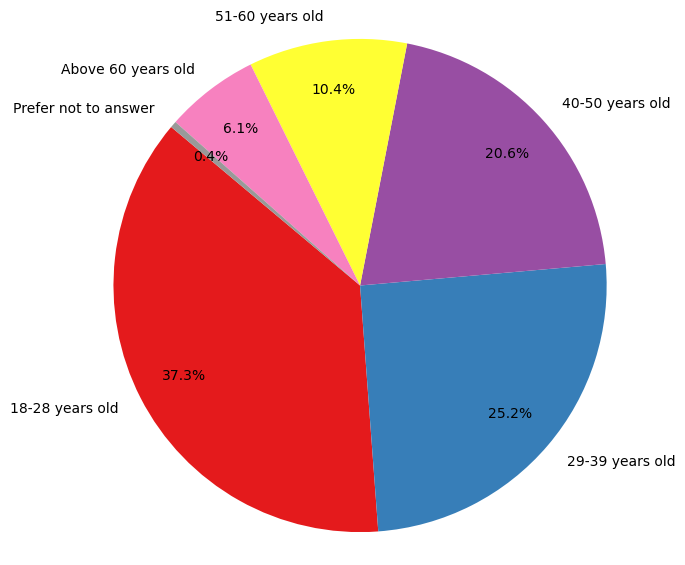
\includegraphics[width=5.7cm]{Age_Distribution.png} % Fixed width
        \caption{Age} % Add your caption here
        \label{fig:Age_Distribution} % Add a label for referencing
    \end{minipage}
    \hfill
    \begin{minipage}[b]{0.3\textwidth} % Adjust width as needed
        \centering
        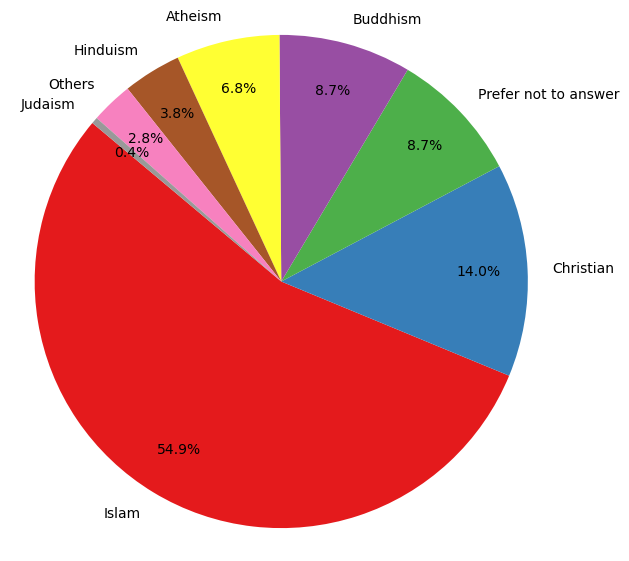
\includegraphics[width=5.18 cm, height=4.7cm] {religion-Distribution} % Fixed width
        \caption{Religion} % Add your caption here
        \label{fig:religion-Distribution} % Add a label for referencing
    \end{minipage}
\end{figure}

Fig.~\ref{fig:COO_Distribution} demonstrates the Country of Origin distribution of respondents. The largest proportions are from UK (33.9\%), followed closely by Malaysia (33.7\%) and Pakistan (32.4\%), indicating a nearly equal representation from these three countries.


Fig.~\ref{fig:PI_Distribution} illustrates the Political Ideology distribution of respondents, with 50.0\% preferring not to answer. Among those who provided their ideology, the largest group is Slightly Liberal (15.7\%), followed by Very Liberal (14.0\%) and Centre-Left (10.2\%). Smaller percentages include Far-Left (8.1\%), Centre-Right (1.5\%), and Far-Right (0.6\%).



Fig.~\ref{fig:ed-Distribution} displays the employment status indicating
 that most respondents are employed full-time (51.3\%). Students represent the second-largest group (23.5\%), followed by self-employed individuals (9.3\%). Smaller categories include part-time employees (4.2\%), retirees and those looking for work (both 3.8\%), homemakers (2.5\%), unemployed (0.8\%), and those who prefer not to disclose their status (0.6\%).

\begin{figure}[H]
    \centering
    \begin{minipage}[b]{0.3\textwidth} % Adjust width as needed
        \centering
        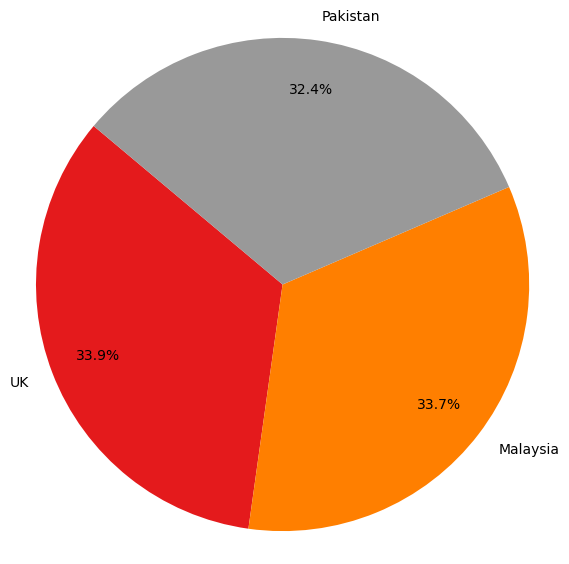
\includegraphics[width=5cm, height=4.85cm]{COO_Distribution.png} % Fixed width
        \caption{Country of Origin} % Add your caption here
        \label{fig:COO_Distribution} % Add a label for referencing
    \end{minipage}
    \hfill
    \begin{minipage}[b]{0.3\textwidth} % Adjust width as needed
        \centering
        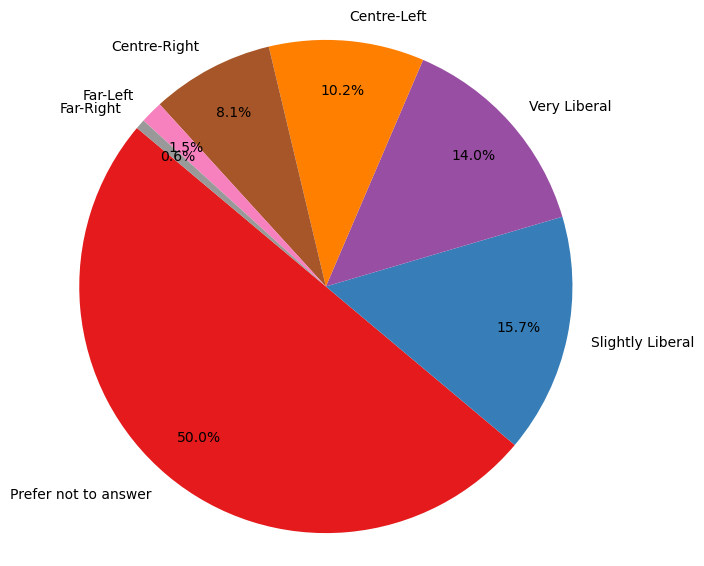
\includegraphics[width=5.8cm, height=4.7cm]{PI_Distribution.png} % Fixed width
        \caption{Political Ideology} % Add your caption here
        \label{fig:PI_Distribution} % Add a label for referencing
    \end{minipage}
    \hfill
    \begin{minipage}[b]{0.3\textwidth} % Adjust width as needed
        \centering
        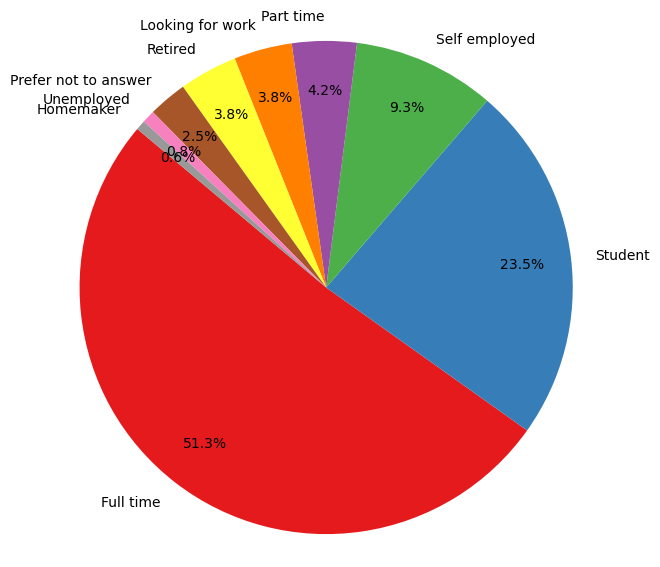
\includegraphics[width=5.6cm, height=4.6cm]{ed-Distribution.png} % Fixed width
        \caption{Employment} % Add your caption here
        \label{fig:ed-Distribution} % Add a label for referencing
    \end{minipage}
\end{figure}

\subsubsection{Partisanship Distribution}

Fig.~\ref{fig:partisanship-distribuiton} shows the Distribution of Partisanship levels among respondents. The majority, 276, are categorized as having Strong Partisanship, while 196 exhibit Weak Partisanship.

Fig.~\ref{fig:partisanship-coo} illustrates the Distribution of Partisanship Level by Country of Origin. In the UK and Pakistan, the majority exhibit Strong Partisanship, with over 100 respondents in each country, while fewer than 50 respondents show Weak Partisanship. In contrast, Malaysia has a more balanced distribution, with a slightly higher number of respondents indicating Weak Partisanship compared to Strong Partisanship.

Fig.~\ref{fig:partisanship-distribuiton-by-employment-status} demonstrates the distribution of partisanship level by employment status. Respondents with full-time employment show the highest counts for both strong partisanship and weak partisanship, with strong partisanship being slightly more common. Students also exhibit high counts for both levels, with strong partisanship dominating. Other employment categories, such as part-time and self-employed, show lower but relatively balanced distributions between the two levels. Categories like homemakers, disabled, and unemployed have minimal representation, while looking for work has slightly more respondents with strong partisanship compared to weak partisanship.

\begin{figure}[H]
    \centering
    % First row: Two graphs
    \begin{minipage}[b]{0.45\textwidth}
        \centering
        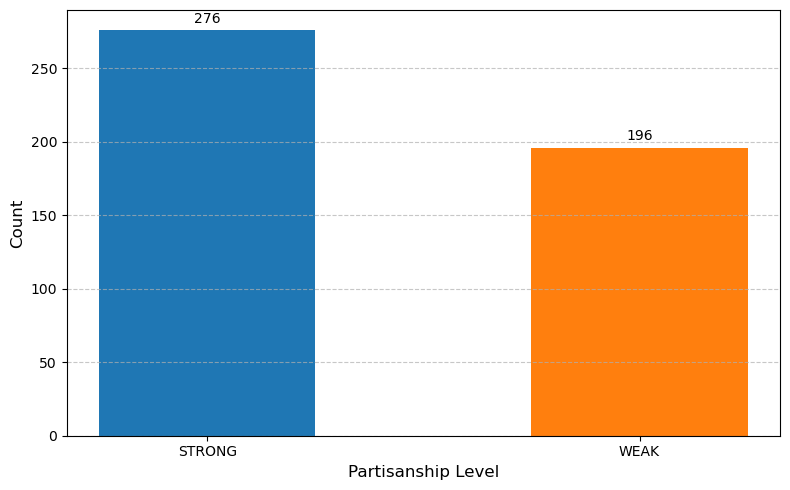
\includegraphics[width=\textwidth]{partisanship-distribuiton.png}
        \caption{Distribution of Partisanship Level} % Add your caption here
        \label{fig:partisanship-distribuiton} % Add a label for referencing
    \end{minipage}
    \hfill
    \begin{minipage}[b]{0.45\textwidth}
        \centering
        \vspace{-20cm}
        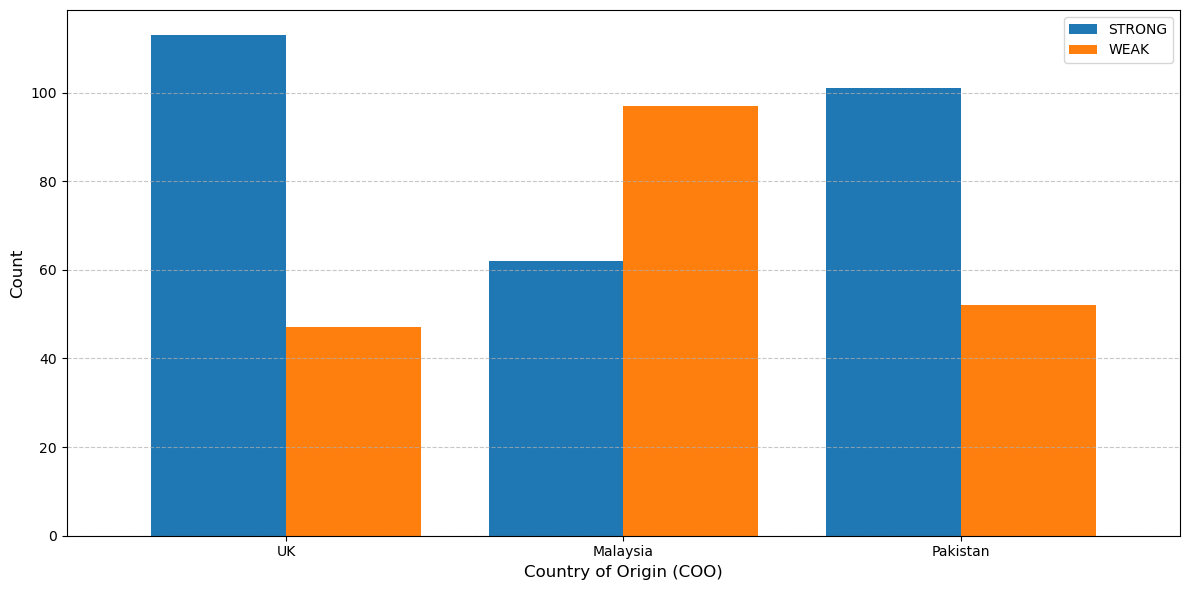
\includegraphics[width=\textwidth, height=4.5cm]{partisanship-distribuiton-by-coo.png}
         \caption{Partisanship by Country of Origin} % Add your caption here
        \label{fig:partisanship-coo} % Add a label for referencing
    \end{minipage}

    \vspace{1cm} % Space between rows

    \centering  
    % Second row: One graph
    \begin{minipage}[b]{0.6\textwidth} % Adjust width as needed
        \centering
        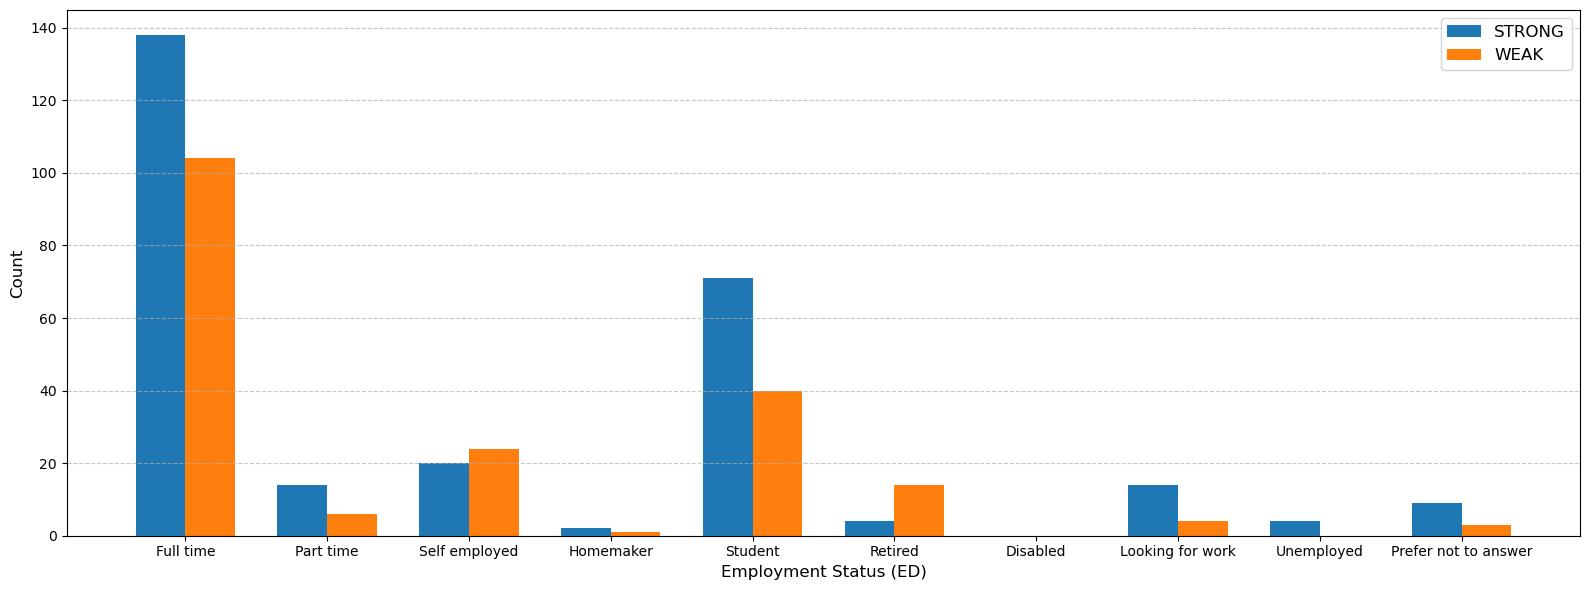
\includegraphics[width=8cm, height=5cm]{partisanship-distribuiton-by-employment-status.png}
        \caption{Partisanship by Employment Status} % Add your caption here
        \label{fig:partisanship-distribuiton-by-employment-status} % Add a label for referencing

    \end{minipage}
\end{figure}
\subsection{\textbf{Data Pre-Processing }}Raw data is often noisy, incomplete or inconsistent, which can hinder the accuracy of machine learning models. To address this issue, several measures have been taken. Firstly, the categorical values from the responses were converted to numerical values according to Table~\ref{tab:table2}. To create the political partisanship scale, feature sets including PS1, PS2, PS3, PS4, PS5, PS6, PS7, PS8, PS9 were merged into a single column named PS-Level. The maximum value obtained for the column was 45 and the lowest value obtained was 9. Thus, we classify the value ranging from 9-26 as 'Weak' class and 27-45 as 'Strong' class. Consequently, we split the data by doing hold-out cross-validation, 80\% of the dataset is used for training and 20\% is reserved for testing.

\begin{table}[H]
\centering
\begin{tabular}{@{}ll@{}}
\toprule
\textbf{Categorical Value} & \textbf{Numerical Value} \\ \midrule
Strongly Disagree          &            1                        \\
Disagree                   &            2                        \\
Neutral                    &            3                        \\
Agree                      &            4                        \\
Strongly Agree             &            5                        \\ \bottomrule

\end{tabular}
\caption{Categorical values encoded with corresponding numerical values }
\label{tab:table2}
\end{table}
\subsubsection{Feature Selection }To ensure the dataset was optimized for model training while avoiding redundancy and irrelevant features, a two-step feature selection process was employed:
\begin{itemize}
    \item \textbf{Pearson's Correlation :} Initially, Pearson’s correlation was calculated for all feature pairs to identify highly correlated features. Highly correlated features generally have no impact on the model's performance. Hence, a threshold of 0.85 was set, beyond which features were considered highly correlated and redundant. Two features exceeded this threshold and were dropped from the dataset resulting in 43 features from 45. Fig.~\ref{fig:figure3} visualizes Pearson's correlation :

% First Figure
\begin{figure}[H]
    \centering
    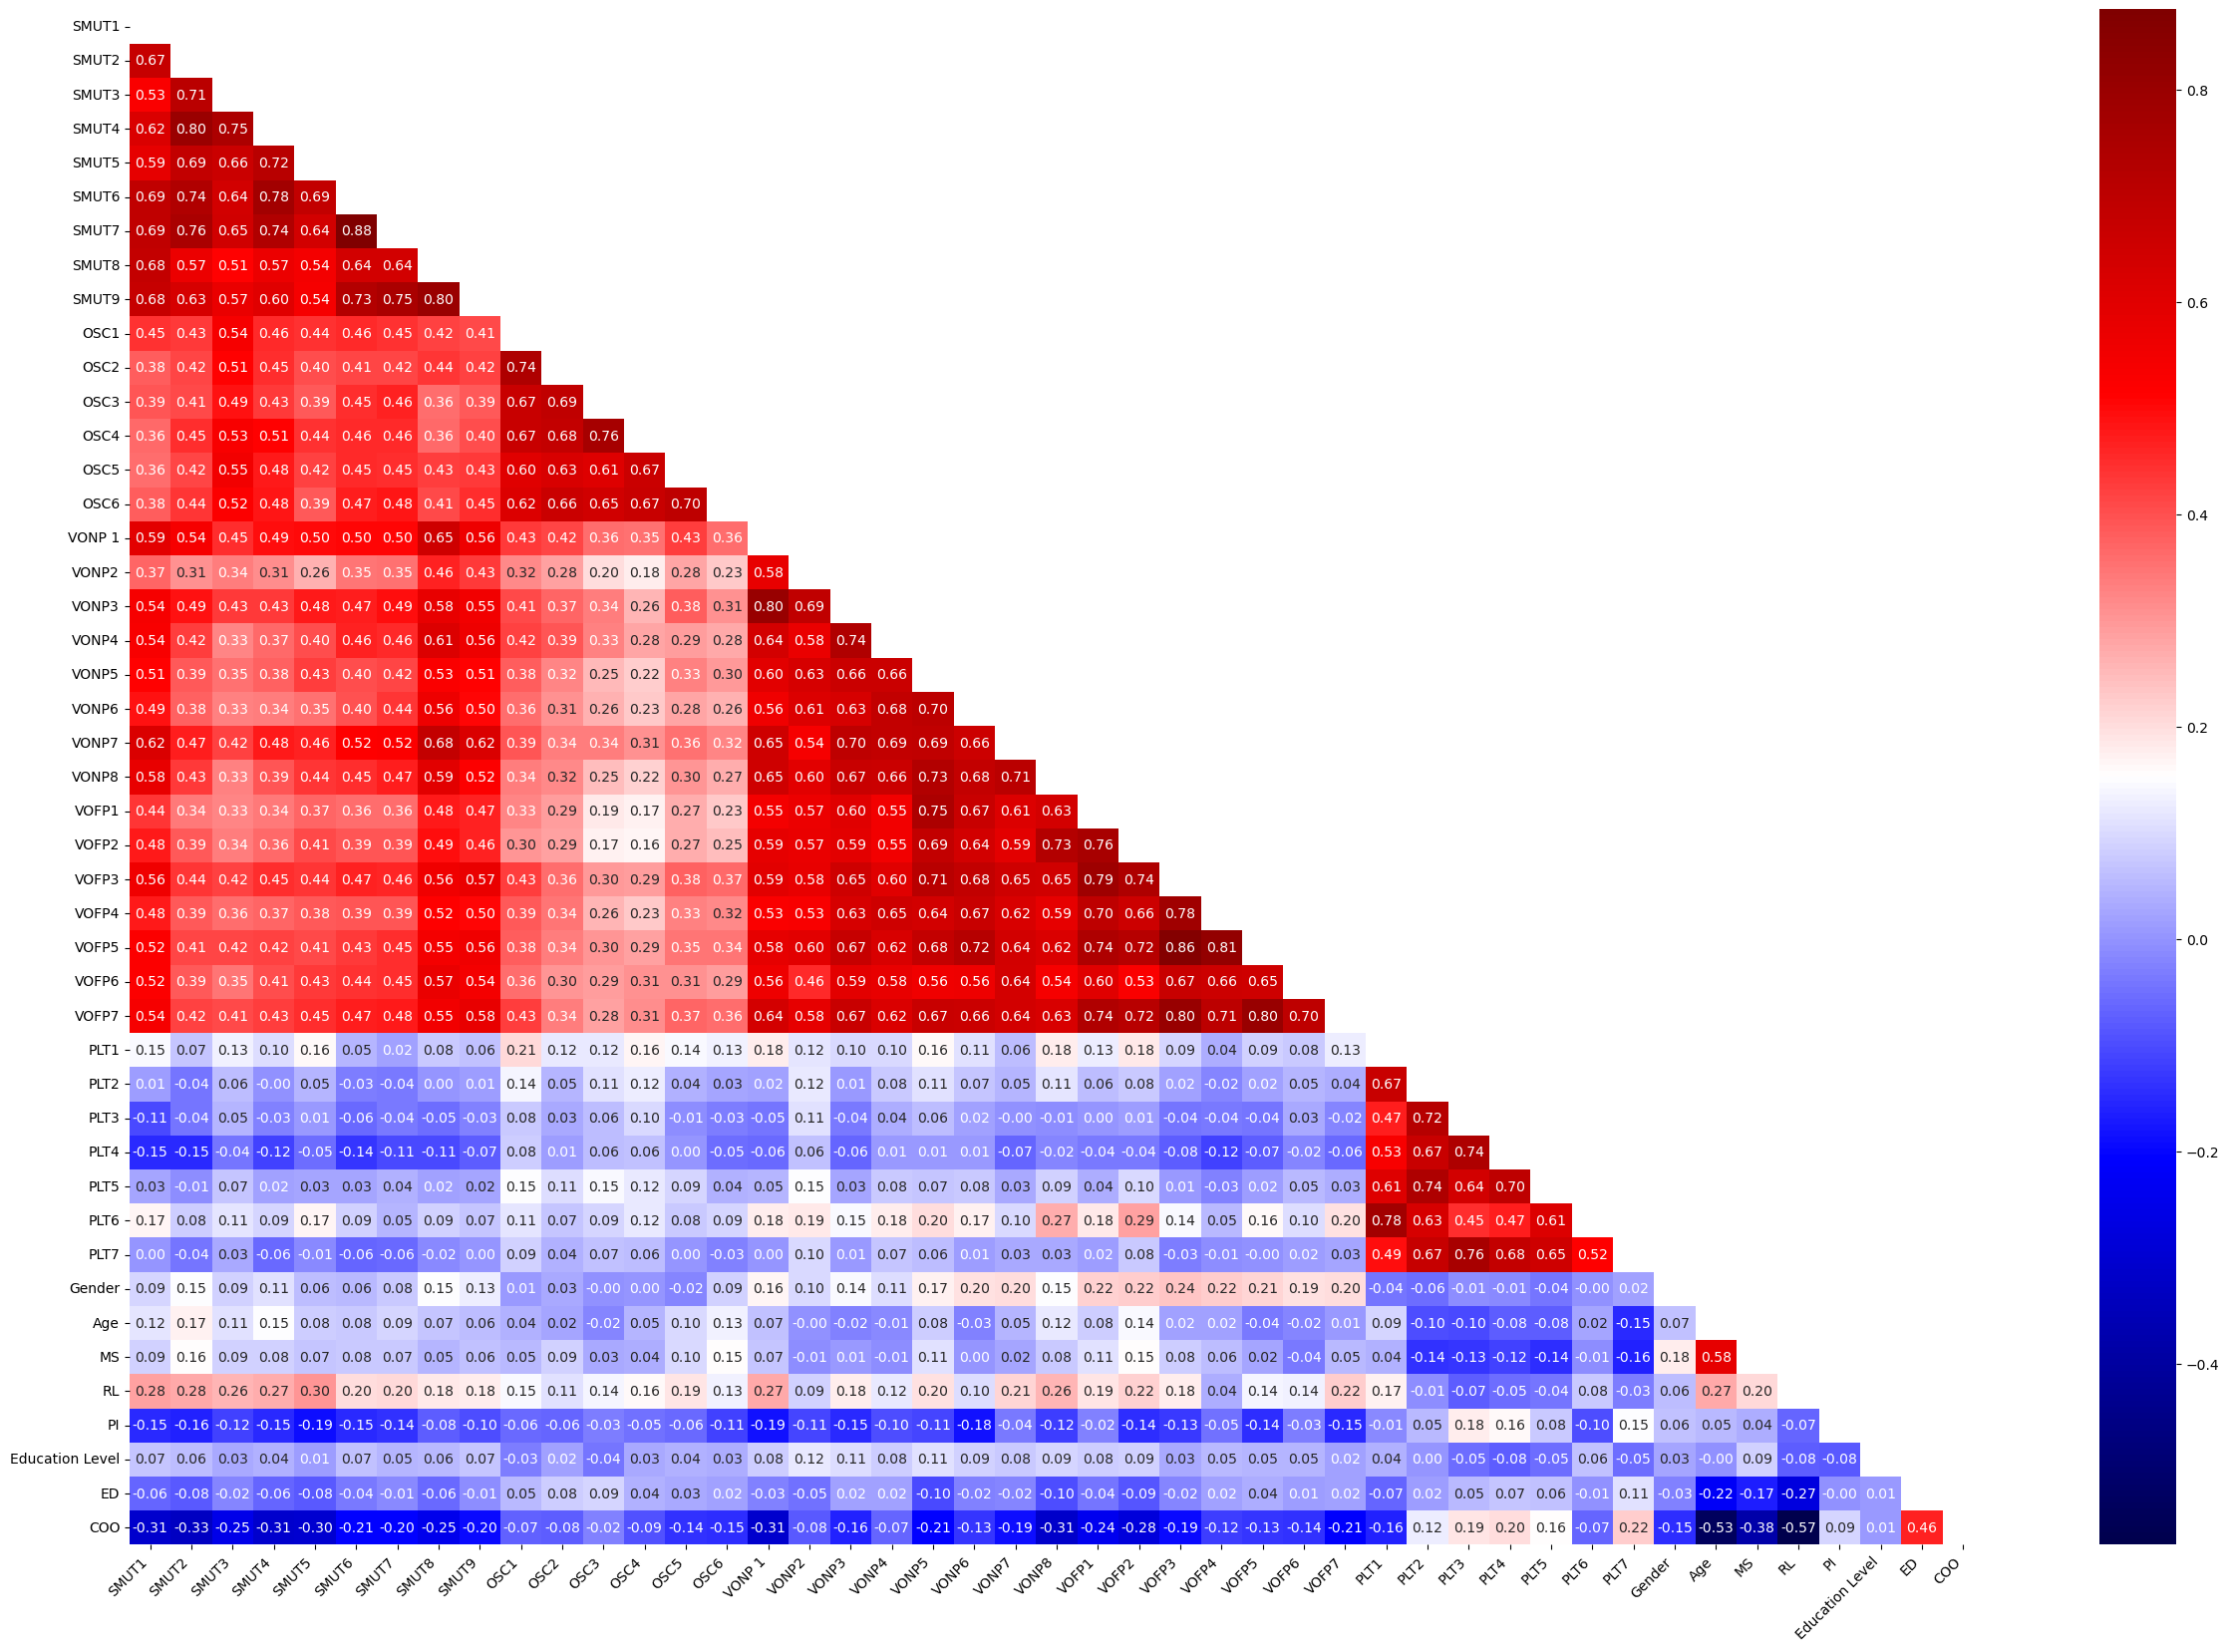
\includegraphics[width=10cm, height=7cm]{Project445/correlation.png} % Replace with your image file
    \caption{\textbf{Correlation Matrix}}
    \label{fig:figure3}
\end{figure}


    \item \textbf{Information Gain :}After removing highly correlated features, the Information Gain algorithm was applied to evaluate the relevance of each feature with respect to the target variable. Here it is used decrease noise of the dataset. Low-scoring features could represent random noise in the dataset rather than meaningful patterns.  A threshold of 0.035 was used, and all features with an information gain below this threshold were removed from the dataset to improve the performance of the model. Below ~\ref{fig:subfig1} shows  the gain scores before dropping the features and ~\ref{fig:subfig2} shows the gain scores after dropping the features : \vspace{0.5cm}

\begin{figure}[h]
    \centering
    % First subfigure
    \begin{subfigure}[b]{0.45\textwidth} % 45% of the text width
        \centering
        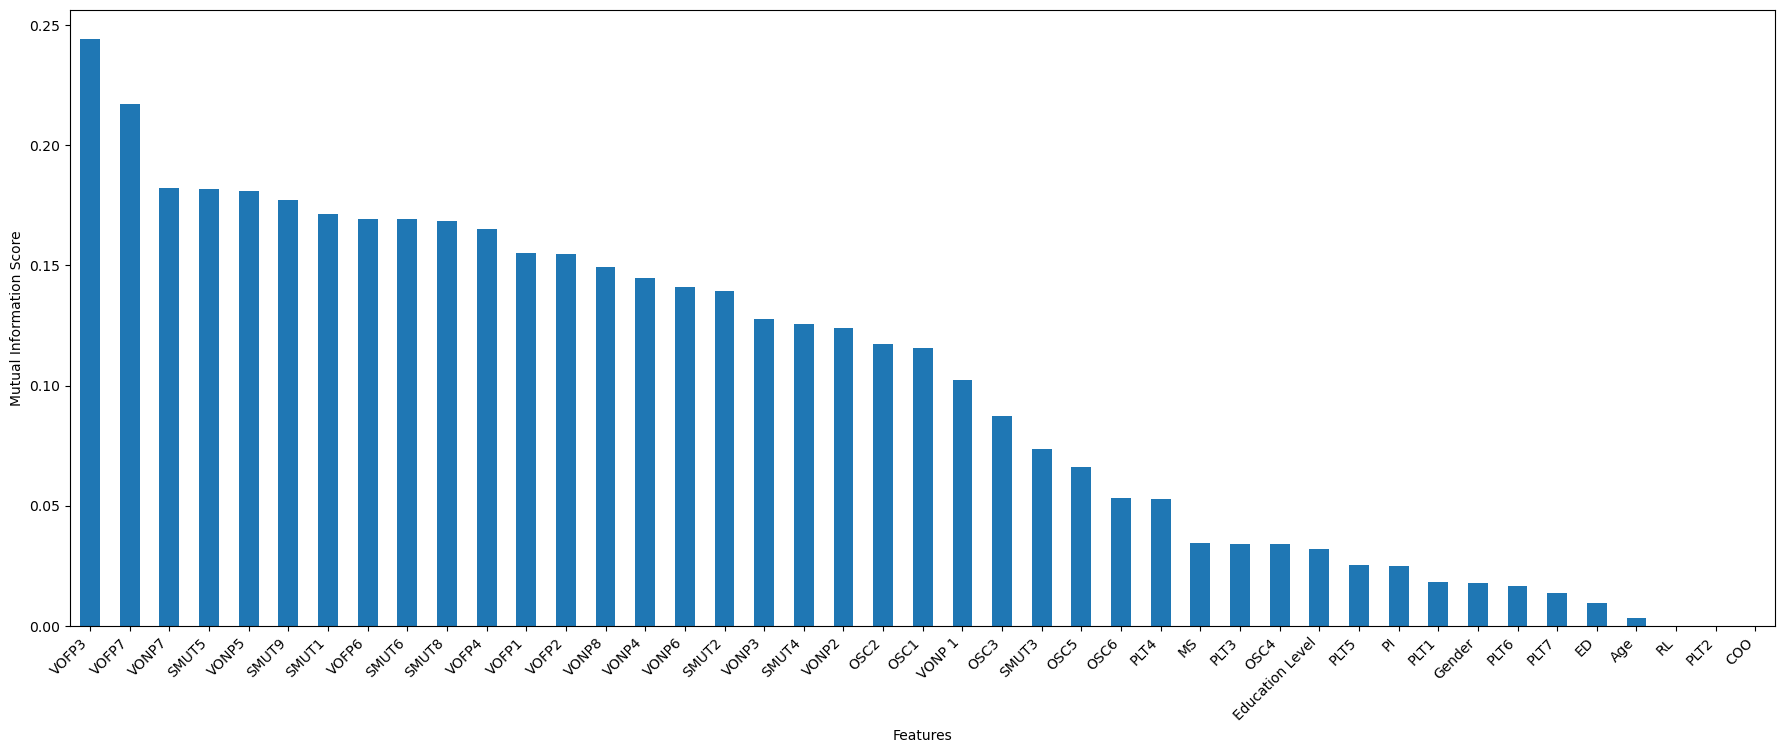
\includegraphics[height=5cm, width=\textwidth]{Project445/information-gain.png}
        \caption{\textbf{Before Threshold Application}}
        \label{fig:subfig1}
    \end{subfigure}
    \hfill % Add some space between the subfigures
    % Second subfigure
    \begin{subfigure}[b]{0.45\textwidth} % 45% of the text width
        \centering
        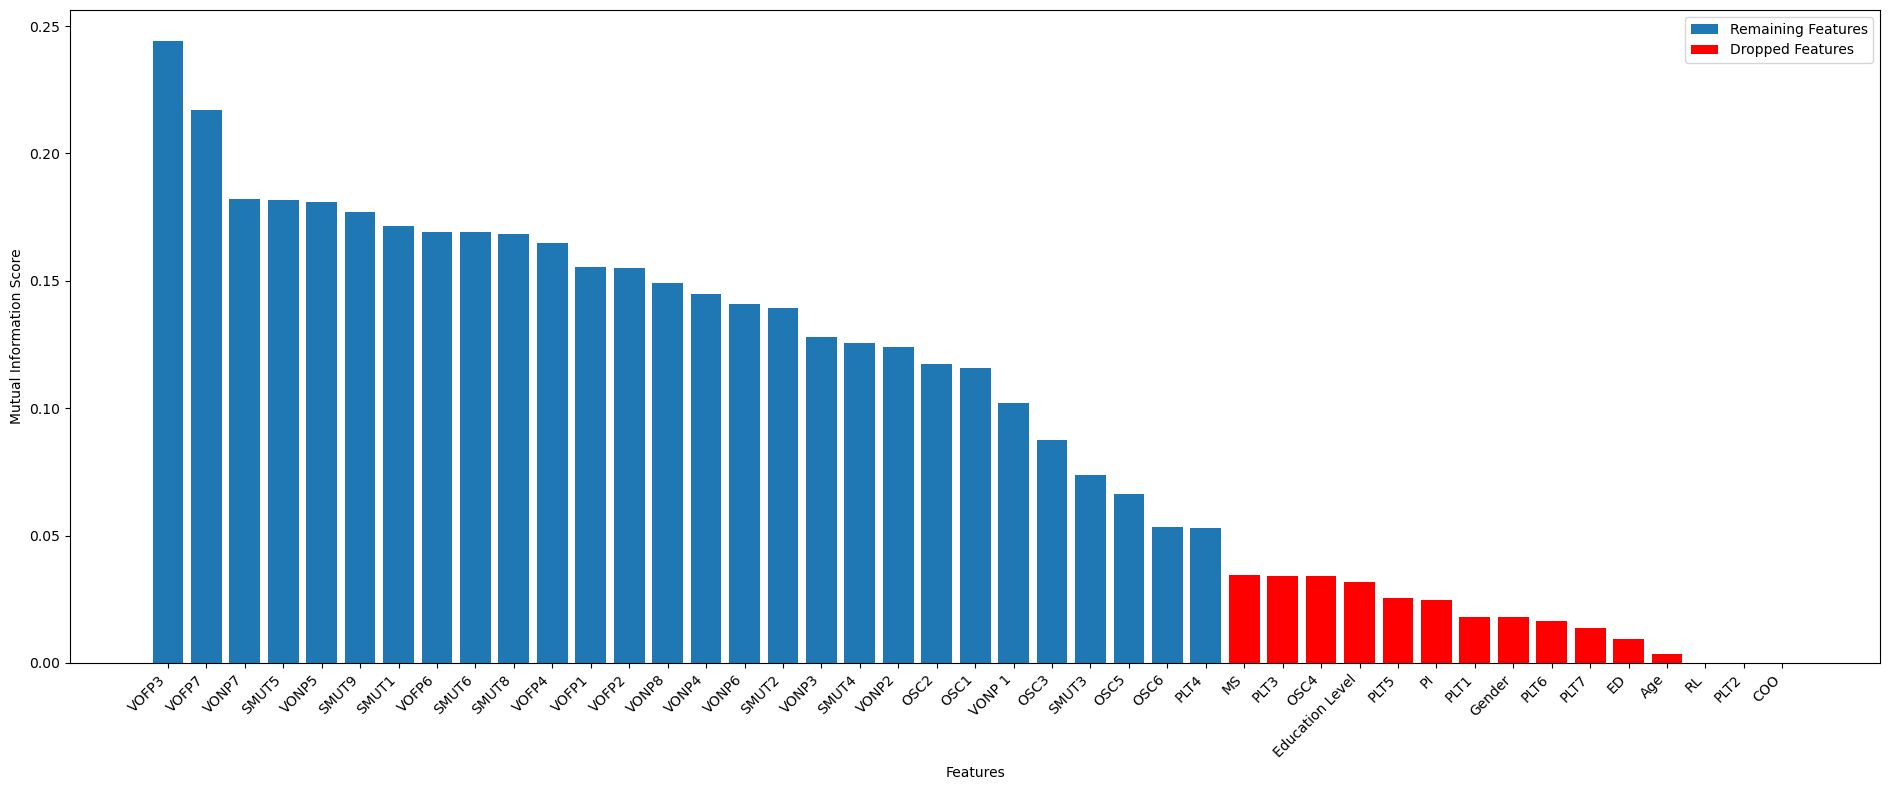
\includegraphics[height=5cm, width=\textwidth]{Project445/ig-red.png} % Replace with your second image file
        \caption{\textbf{After Threshold Application}}
        \label{fig:subfig2}
    \end{subfigure}
    % Overall caption
    \caption{\textbf{Information Gain Scores}}
    \label{fig:figure}
\end{figure}
    
\end{itemize} 

\section{Machine Learning Classifiers with Hyperparameter Tuning}
Once the data is preprocessed, it is divided into train set(80\%) and test set(20\%). Essential Machine learning algorithms, starting with baseline classifiers, Decision Tree, K-Nearest Neighbors (KNN), Support Vector Machine (SVM), Naive Bayes, Logistic Regression and Ensemble classifiers such as Random Forest, AdaBoost, Gradient Boosting, CatBoost and lastly Neural Network by Artificial Neural Network (ANN).

After applying these baseline classifiers and decision-making algorithms, performance evaluation was conducted using metrics such as accuracy, precision, recall, F1-score, and the area under the ROC curve (AUC). Among the ensemble methods, CatBoost stood out as the best performer, achieving the highest accuracy of 87.4\%. CatBoost, a gradient boosting algorithm specifically designed to handle categorical features efficiently, demonstrated exceptional stability and accuracy by leveraging powerful tree-based learning techniques. Its ability to minimize overfitting and handle categorical variables automatically played a crucial role in its success. Advanced models like Artificial Neural Networks (ANN) were also employed to capture complex patterns in the data, leveraging hidden layers to perform non-linear transformations. 

To enhance the performance of the model, hyperparameter optimization is performed primarily on the baseline classifiers. For this purpose, GridSearchCV technique is applied to systematically explore the optimal parameter combinations for each baseline model. Table~\ref{tab:table3} includes the hyperparameter results :\vspace{0.5cm}

\begin{table}[htbp]
    \centering
     \begin{tabular}{|l|p{10cm}|} % Adjust the width as needed
        \hline
        \textbf{Baseline Classifiers} & \textbf{Best Parameters} \\ \hline
        Decision Tree & \texttt{criterion = 'entropy', max\_depth = 10, min\_samples\_split = 2, random\_state = 28} \\ \hline
        K-Nearest Neighbors (KNN) & \texttt{metric = 'euclidean', n\_neighbors = 9, weights = 'uniform'} \\ \hline
        Support Vector Machine (SVM) & \texttt{C = 1, gamma = 'auto', kernel = 'rbf'} \\ \hline
        Naive Bayes & \texttt{var\_smoothing = 1.0} \\ \hline
        Logistic Regression & \texttt{C = 0.01, max\_iter = 500, random\_state = 20, solver = 'lbfgs'} \\ \hline
        \textbf{Ensemble Learning} & \textbf{Selected Parameters} \\ \hline
        Random Forest & \texttt{max\_depth = 10, min\_samples\_split =  10, n\_estimators = 100, random\_state = 29} \\ \hline
        AdaBoost & \texttt{estimator=DecisionTreeClassifier(max\_depth=3, random\_state=42),
    learning\_rate=0.01,
    n\_estimators=50,
    algorithm="SAMME",
    random\_state=42} \\ \hline
        Gradient Boosting & \texttt{learning\_rate = 0.01, max\_depth = 3, n\_estimators = 50, random\_state= 29} \\ \hline
        CatBoost & \texttt{depth= 10, iterations= 100, learning\_rate= 0.1, random\_state= 45, verbose=0} \\ \hline
        \textbf{Neural Network} & \textbf{Selected Parameters} \\
        \hline
        Artificial Neural Network (ANN) & \texttt{hidden\_layer\_sizes=(120,70), max\_iter=1000, random\_state=22} \\ \hline
       
    \end{tabular}
    \caption{Best Combination of Parameters}
    \label{tab:table3}
\end{table}

\section{Result Analysis}
The performance metrics for different classifiers, including Accuracy, Precision, Recall, and F1 Score, were evaluated to evaluate the effectiveness of the models in predicting "Strong" and "Weak" classes. The results are summarized in Table~\ref{tab:classifiers_performance}. As a benchmark for other classification methods. ZeroR classifier is applied first that obtained 55\% accuracy. Other classifiers, like the Decision Tree, Random Forest, and Boosting methods (AdaBoost, Gradient Boost, and CatBoost) did much better than the decision tree-based models. With an accuracy of 87\%, the CatBoost algorithm had the best precision (0.84 for "Strong" and 0.92 for "Weak") and F1 Scores (0.89 and 0.85 for "Strong" and "Weak," respectively). The Random Forest and AdaBoost models also achieved strong results, with accuracies of 85\% and balanced performance across all metrics. Algorithms like,Naive Bayes achieved an accuracy of 86\%, with an F1 Score of 0.88 for "Strong" and 0.85 for "Weak," indicating its strength in handling the class imbalance. K-Nearest Neighbor (KNN) and logistic regression both performed well, with accuracies of 82\% and 84\%, respectively, although they fell somewhat short of boosting techniques in terms of recall for the "Weak" class. The Support Vector Machine (SVM) classifier had an 81\% accuracy rate, with a little bias towards the "Strong" class in both precision and recall. It performed satisfactorily overall, but its F1 Score for the "Weak" class (0.76) was significantly lower. With an accuracy of 85\% and balanced precision, recall, and F1 Scores across both classes, the Artificial Neural Network (ANN) concluded by demonstrating superior performance. An overall look at the results shows that ensemble methods, especially CatBoost, offered the most satisfactory accuracy and performance across all metrics. 



\begin{table}[H]
\centering
\begin{tabular}{|c|c|cc|cc|cc|}
\hline
\textbf{Classifier} & \textbf{Accuracy} & \multicolumn{2}{c|}{\textbf{Precision}} & \multicolumn{2}{c|}{\textbf{Recall}} & \multicolumn{2}{c|}{\textbf{F1 Score}} \\ \cline{3-8} 
                    &                   & \textbf{Strong}    & \textbf{Weak}    & \textbf{Strong}    & \textbf{Weak}   & \textbf{Strong}    & \textbf{Weak}    \\ \hline
Zero-R        & 0.55              & 0.55               & 0.00             & 1.00               & 0.00            & 0.71               & 0.00             \\ \hline
Decision Tree        & 0.84              & 0.81               & 0.89             & 0.92               & 0.74            & 0.86               & 0.81             \\ \hline
K-Nearest Neighbor (KNN)       & 0.84              & 0.80               & 0.91             & 0.94               & 0.72            & 0.87               & 0.81             \\ \hline
Logistic Regression        & 0.82              & 0.81               & 0.84             & 0.88               & 0.74            & 0.84               & 0.79             \\ \hline
Naive Bayes        & 0.86              & 0.87               & 0.86             & 0.88               & 0.84            & 0.88               & 0.85             \\ \hline
Support Vector Machine (SVM)        & 0.81              & 0.77               & 0.88             & 0.92               & 0.67            & 0.84               & 0.76             \\ \hline
Random Forest       & 0.85              & 0.83               & 0.89             & 0.92               & 0.77            & 0.87               & 0.82             \\ \hline
AdaBoost        & 0.85              & 0.82               & 0.91             & 0.94               & 0.74            & 0.88               & 0.82             \\ \hline
Gradient Boost        & 0.82              & 0.78               & 0.91             & 0.94               & 0.67            & 0.85               & 0.77             \\ \hline
CatBoost       & 0.87              & 0.84               & 0.92             & 0.94               & 0.79            & 0.89               & 0.85             \\ \hline
Artificial Neural Network (ANN)       & 0.85              & 0.85               & 0.85             & 0.88               & 0.81            & 0.87               & 0.83             \\ \hline
\end{tabular}
\caption{Performance Metrics for Different Classifiers}
\label{tab:classifiers_performance}
\end{table}


\subsection{Confusion Matrix}
Here, the confusion matrices summarizes the model's performance by showing the counts of correct and incorrect predictions across classes. It highlights True Positives, True Negatives, False Positives, and False Negatives, providing insights into accuracy and error distribution\cite{ref11}. Fig~\ref{fig:con-figure} shows the confusion matrices of the models. CatBoost  provided the most promising result than others. It is able to classify 53 Strong classes and 34 Weak classes correctly. However, 3 Strong classes are classified as Weak and 5 Weak class as Strong. Hence, 8 instances are miss classified being the lowest among other models.

\begin{figure}[H]
\begin{center}
% First row: 3 images
\begin{tabular}{c c c} % Three centered columns
    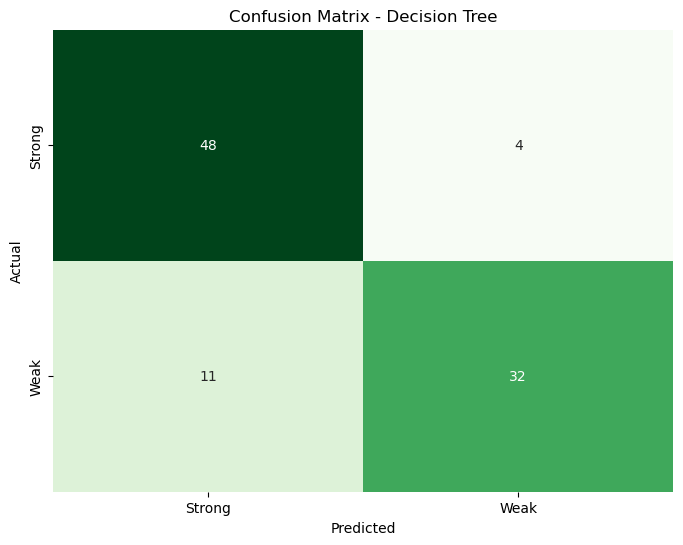
\includegraphics[width=0.35\textwidth]{confusion-matrix/decision-tree.png} & % Adjust width to fit
    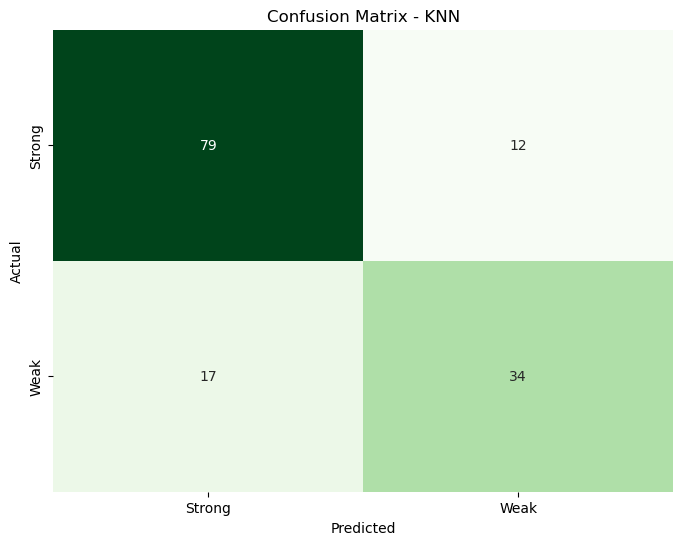
\includegraphics[width=0.35\textwidth]{confusion-matrix/knn.png} &
    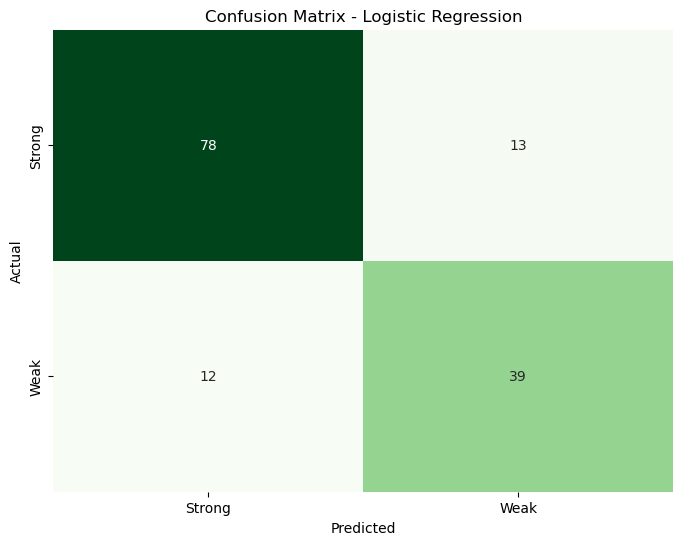
\includegraphics[width=0.35\textwidth]{confusion-matrix/logistic.png} \\
\end{tabular}

\vspace{5pt} % Adjust spacing between rows

% Second row: 2 images
\begin{tabular}{c c} % Two centered columns
    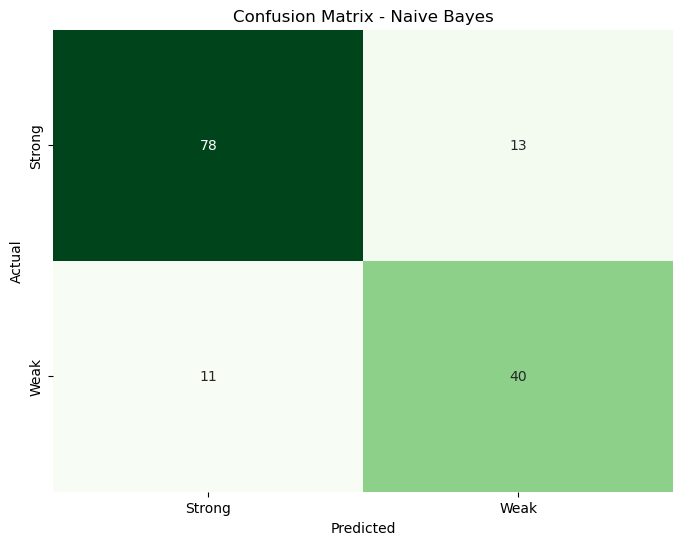
\includegraphics[width=0.35\textwidth]{confusion-matrix/naive-bayes.png} &
    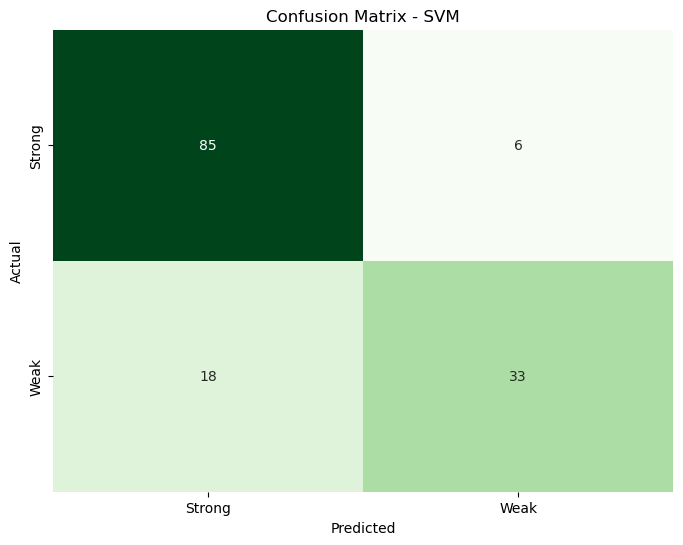
\includegraphics[width=0.35\textwidth]{confusion-matrix/svm.png} \\
\end{tabular}

\vspace{5pt} % Adjust spacing between rows

% Third row: 3 images
\begin{tabular}{c c c} % Three centered columns
    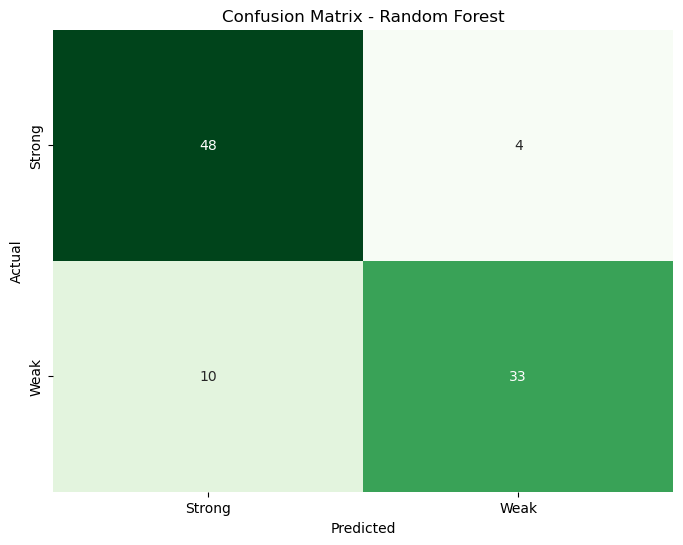
\includegraphics[width=0.35\textwidth]{confusion-matrix/rf.png} &
    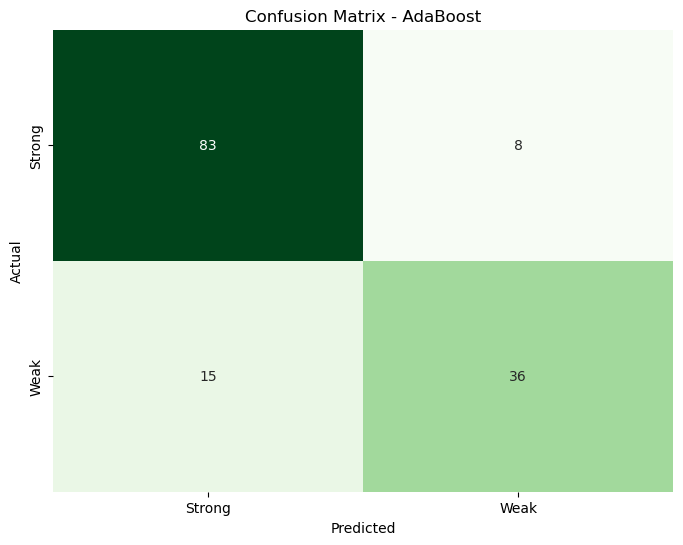
\includegraphics[width=0.35\textwidth]{confusion-matrix/adaboost.png} &
    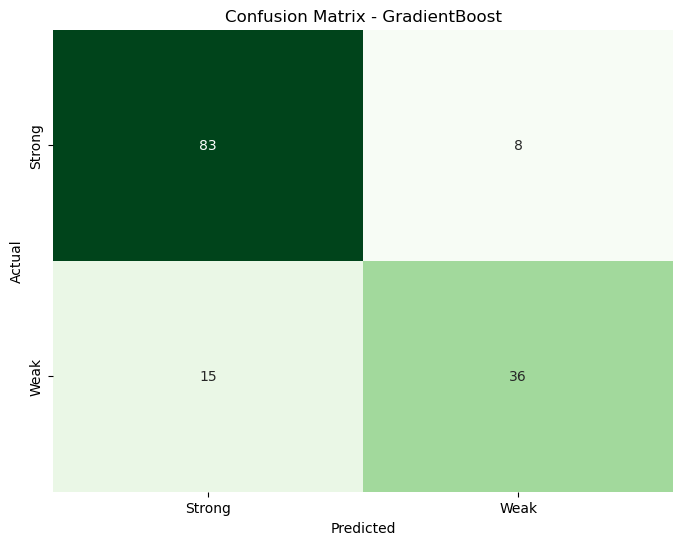
\includegraphics[width=0.35\textwidth]{confusion-matrix/gboost.png} \\
\end{tabular}

\vspace{5pt} % Adjust spacing between rows

% Fourth row: 2 images
\begin{tabular}{c c} % Two centered columns
    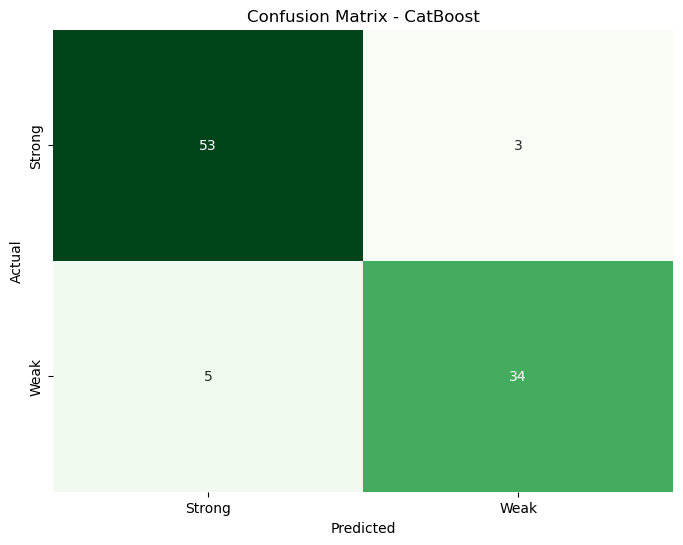
\includegraphics[width=0.35\textwidth]{confusion-matrix/catboost.png} &
    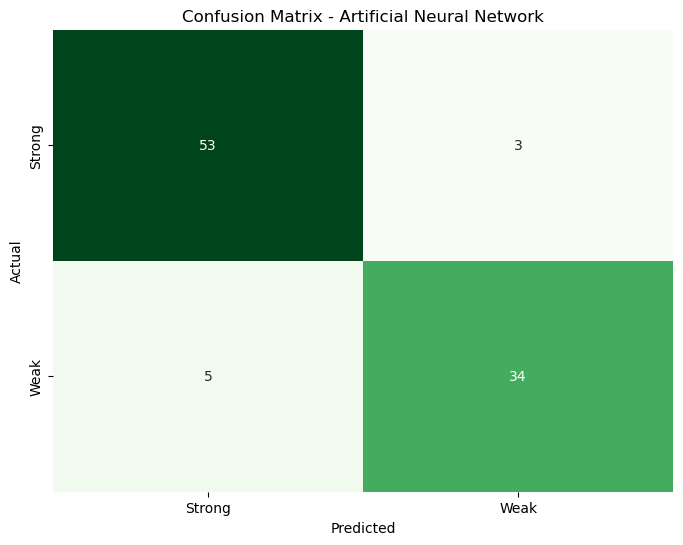
\includegraphics[width=0.35\textwidth]{confusion-matrix/ann.png} \\
\end{tabular}

\end{center}
    \caption{\textbf{Confusion Matrix of Different Classifiers}}
    \label{fig:con-figure} 
\end{figure}

\subsection{Receiver Operating Characteristic (ROC) Curve}

The ROC curve is a graphical representation of a classification model's performance across different threshold values. A higher AUC value (closer to 1.0) reflects better discrimination ability, while a curve closer to the diagonal (AUC $\approx$ 0.5) represents poor or random performance\cite{ref12}. Fig~\ref{fig:roc-figure} shows that most models demonstrate strong classification performance, as evident from their high AUC scores and curves well above the diagonal baseline, with slight variations in the sharpness and smoothness of the curves depending on the model's complexity and optimization. These results suggest that the dataset and selected features are effective for predicting partisanship across multiple algorithms.


\begin{figure}[H]
\begin{center}
% First row: 3 images
\begin{tabular}{c c c} % Three centered columns
    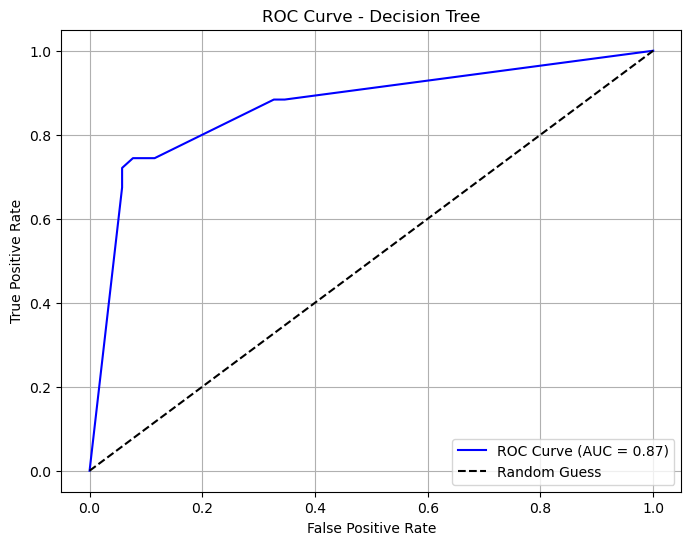
\includegraphics[width=0.35\textwidth]{roc-curve/decision-tree.png} & % Adjust width to fit
    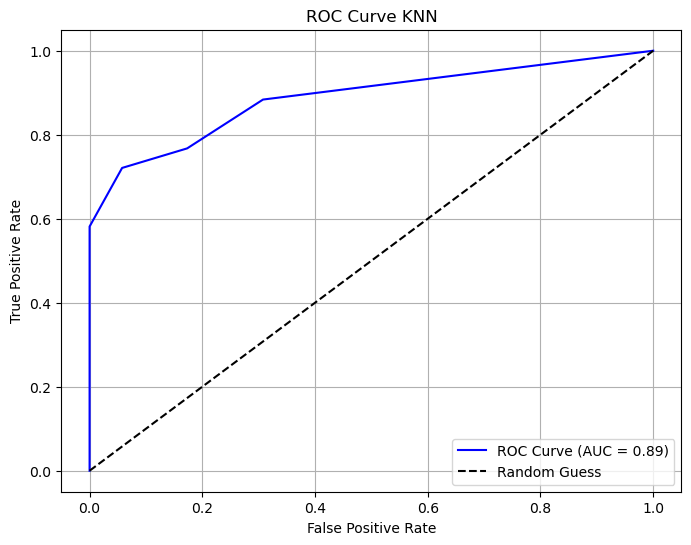
\includegraphics[width=0.35\textwidth]{roc-curve/knn.png} &
    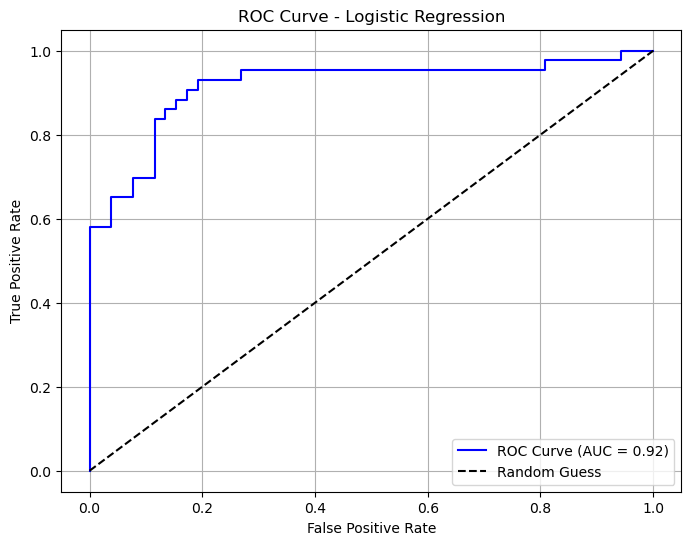
\includegraphics[width=0.35\textwidth]{roc-curve/logistic.png} \\
\end{tabular}

\vspace{5pt} % Adjust spacing between rows

% Second row: 2 images
\begin{tabular}{c c} % Two centered columns
    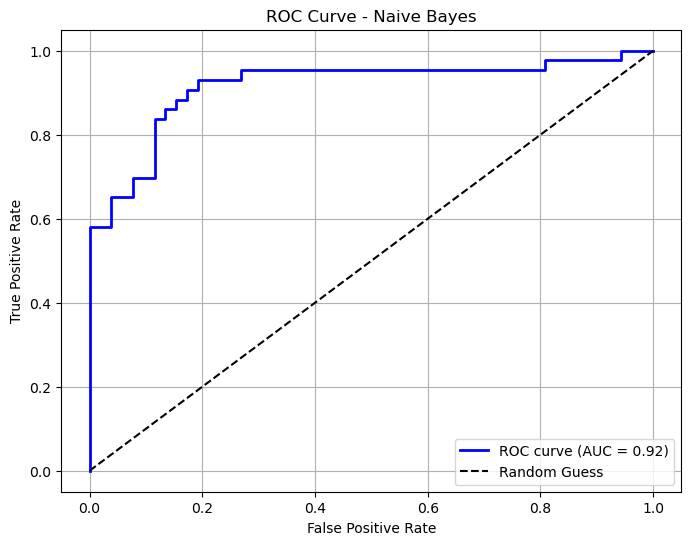
\includegraphics[width=0.35\textwidth]{roc-curve/nb.png} &
    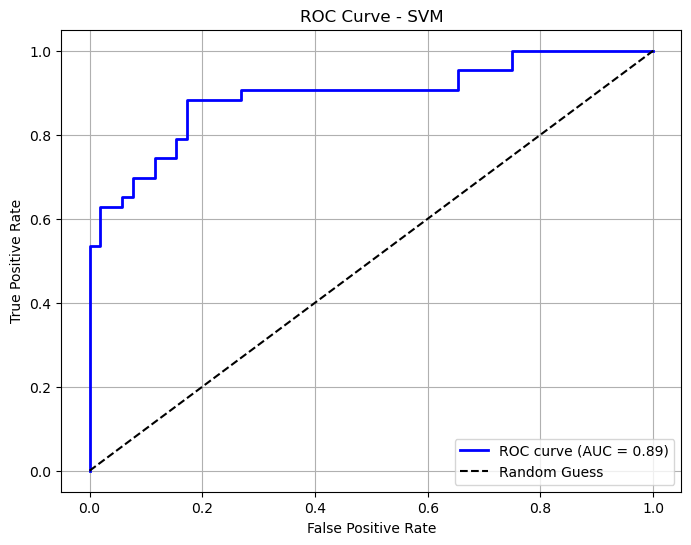
\includegraphics[width=0.35\textwidth]{roc-curve/svm.png} \\
\end{tabular}

\vspace{5pt} % Adjust spacing between rows

% Third row: 3 images
\begin{tabular}{c c c} % Three centered columns
    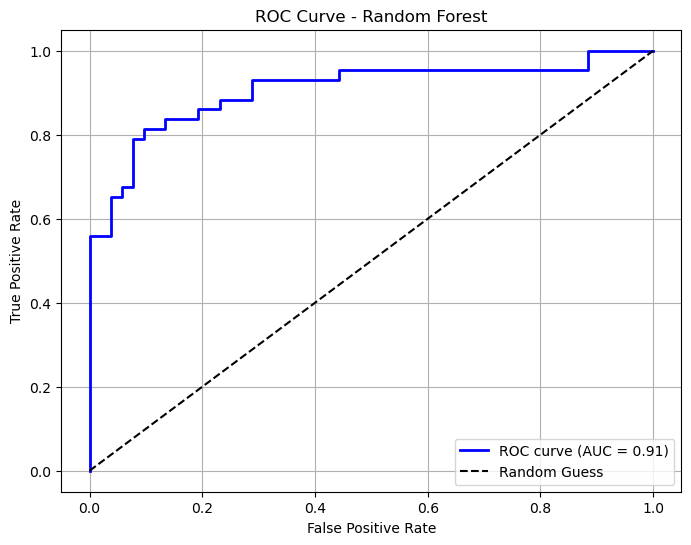
\includegraphics[width=0.35\textwidth]{roc-curve/rf.png} &
    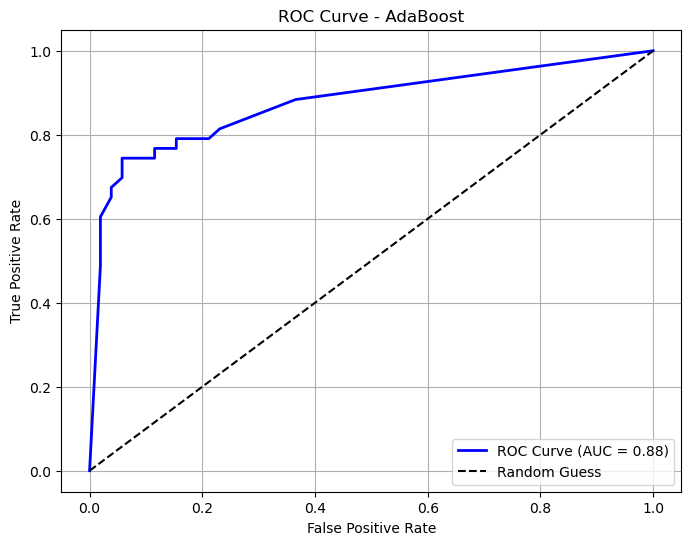
\includegraphics[width=0.35\textwidth]{roc-curve/ada.png} &
    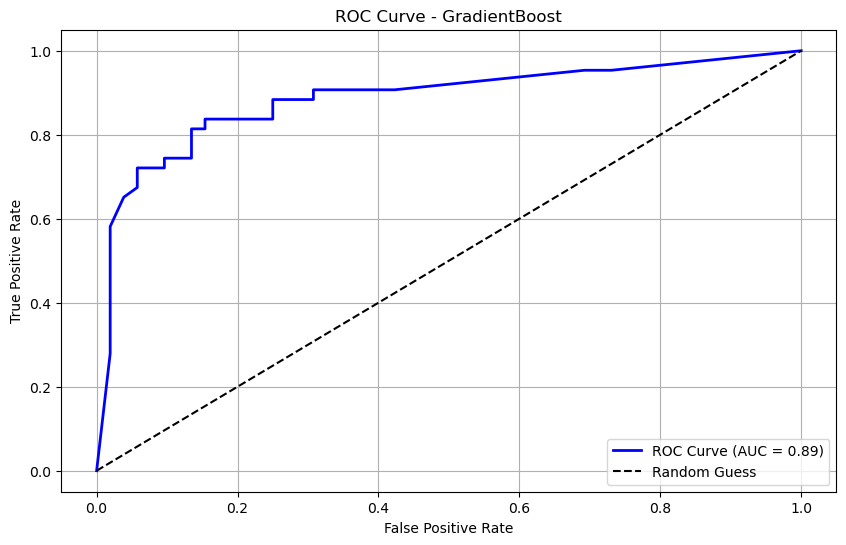
\includegraphics[width=0.34\textwidth,height = 4.5cm]{roc-curve/gb.png} \\
\end{tabular}

\vspace{5pt} % Adjust spacing between rows

% Fourth row: 2 images
\begin{tabular}{c c} % Two centered columns
    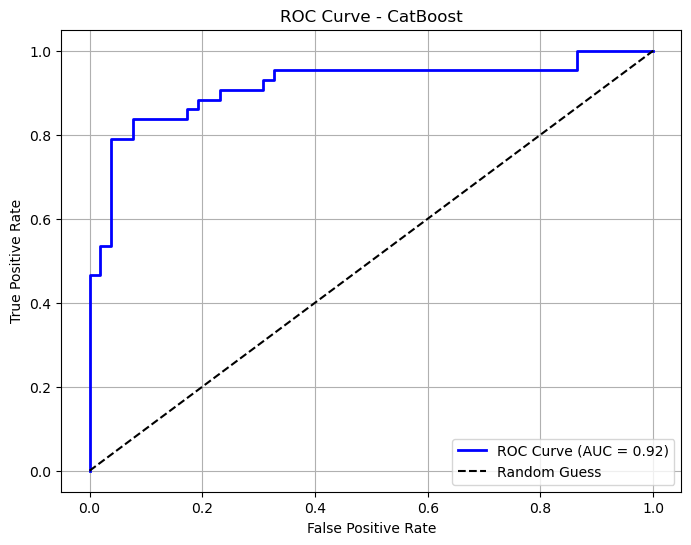
\includegraphics[width=0.35\textwidth]{roc-curve/cb.png} &
    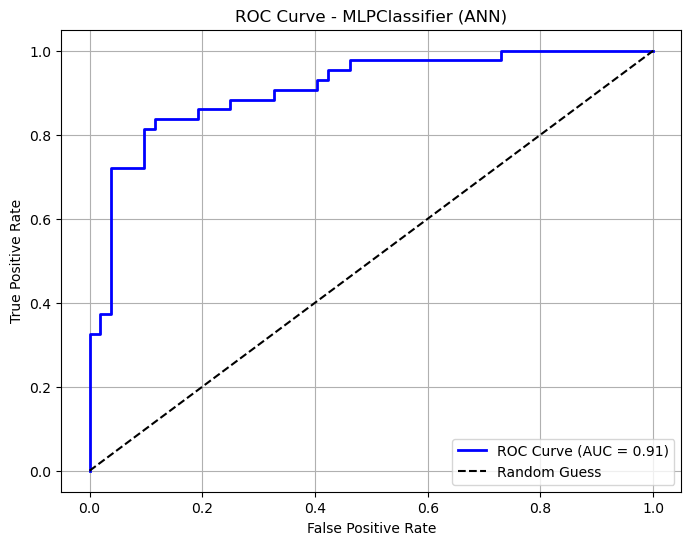
\includegraphics[width=0.35\textwidth]{roc-curve/ann.png} \\
\end{tabular}
\end{center}
    \caption{\textbf{ROC Curves of Different Classifiers}}
    \label{fig:roc-figure} 
\end{figure}

\subsection{Precision-Recall Curve (PRC)}
The PRC (Precision-Recall Curve) shows the trade-off between precision and recall, highlighting a model's effectiveness in handling positive cases. PRC can be more informative than other performance matrices for binary classification\cite{ref13}. Fig~\ref{fig:prc-figure} includes the precision-recall curves of different models :

\begin{figure}[H]
\begin{center}
% First row: 3 images
\begin{tabular}{c c c} % Three centered columns
    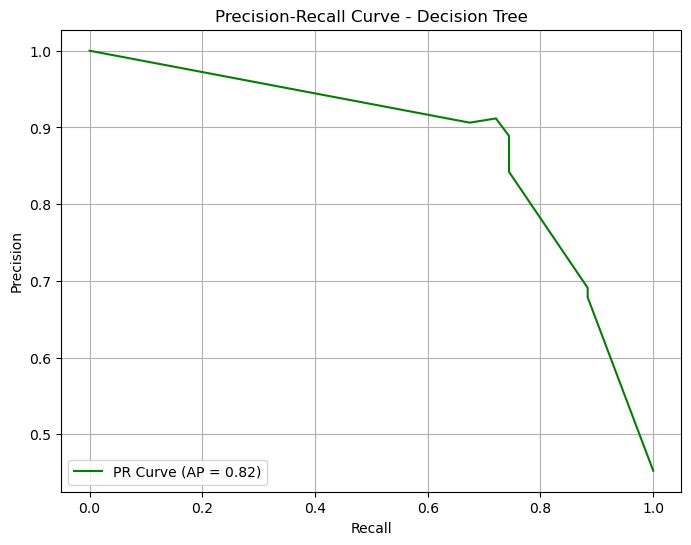
\includegraphics[width=0.35\textwidth]{prc-curve/decision.png} & 
    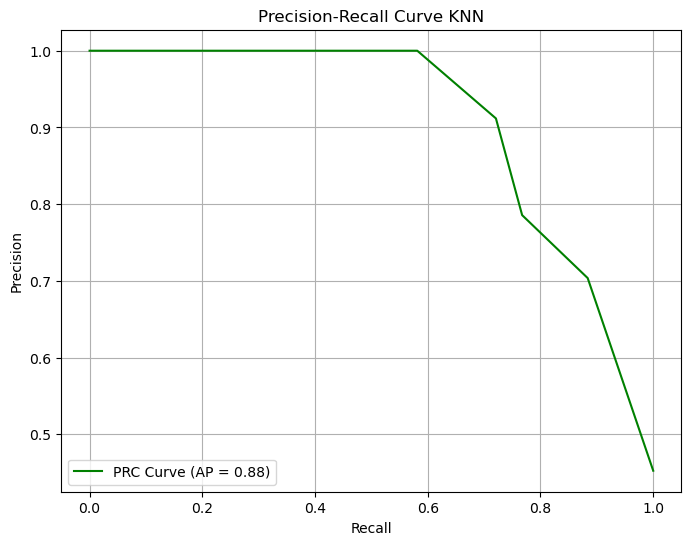
\includegraphics[width=0.35\textwidth]{prc-curve/knn.png} &
    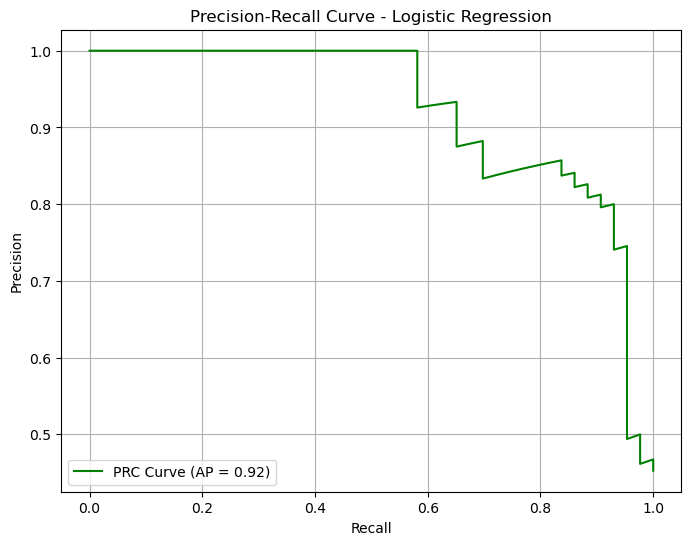
\includegraphics[width=0.35\textwidth]{prc-curve/logistic.png} \\
\end{tabular}

\vspace{5pt} % Adjust spacing between rows

% Second row: 2 images
\begin{tabular}{c c} % Two centered columns
    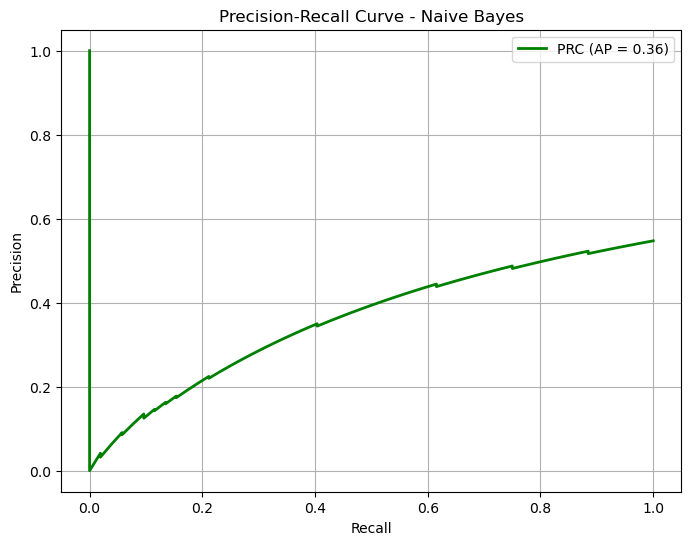
\includegraphics[width=0.35\textwidth]{prc-curve/nb.png} &
    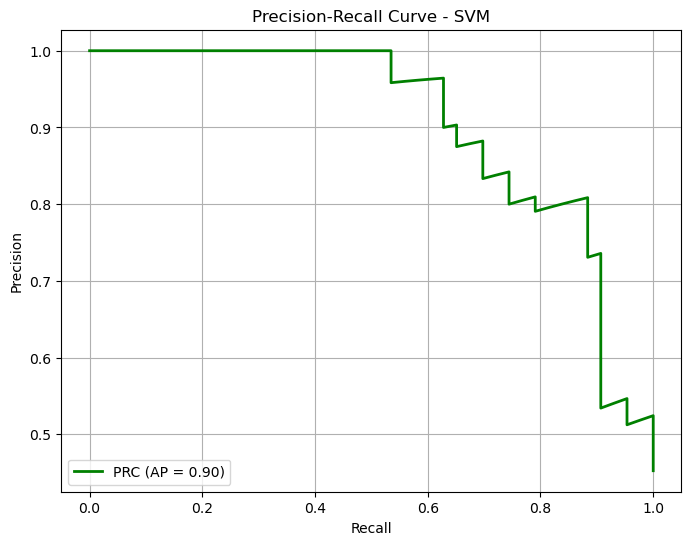
\includegraphics[width=0.35\textwidth]{prc-curve/svm.png} \\
\end{tabular}

\vspace{5pt} % Adjust spacing between rows

% Third row: 3 images
\begin{tabular}{c c c} % Three centered columns
    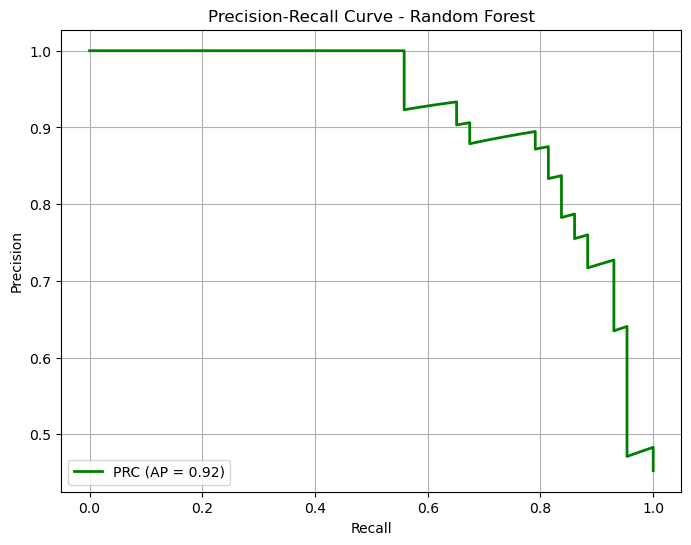
\includegraphics[width=0.35\textwidth]{prc-curve/rf.png} &
    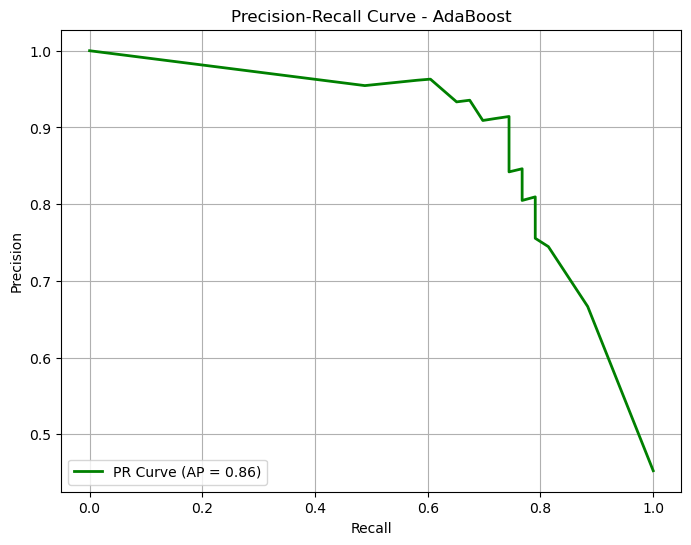
\includegraphics[width=0.35\textwidth]{prc-curve/ada.png} &
    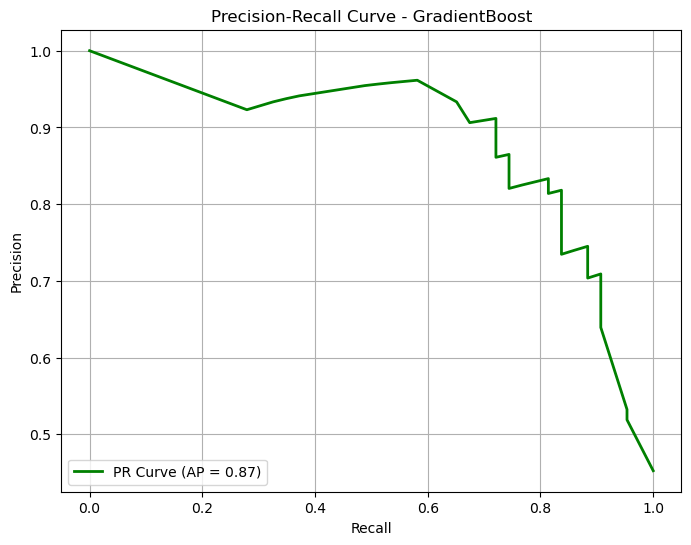
\includegraphics[width=0.35\textwidth]{prc-curve/gb.png} \\
\end{tabular}

\vspace{5pt} % Adjust spacing between rows

% Fourth row: 2 images
\begin{tabular}{c c} % Two centered columns
    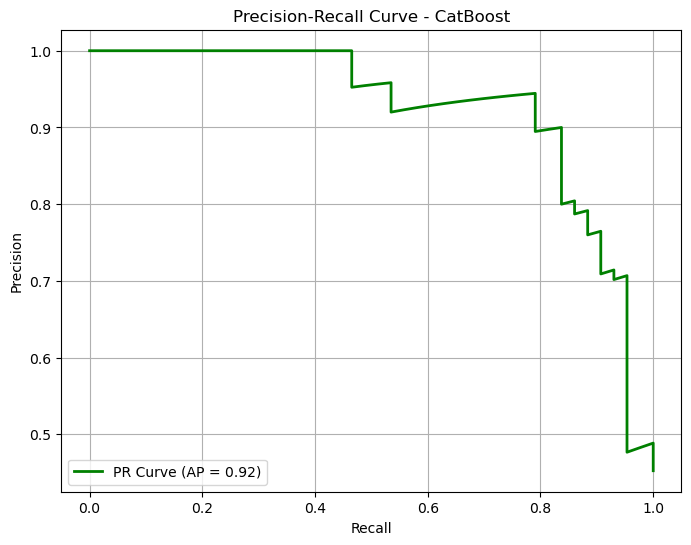
\includegraphics[width=0.35\textwidth]{prc-curve/cb.png} &
    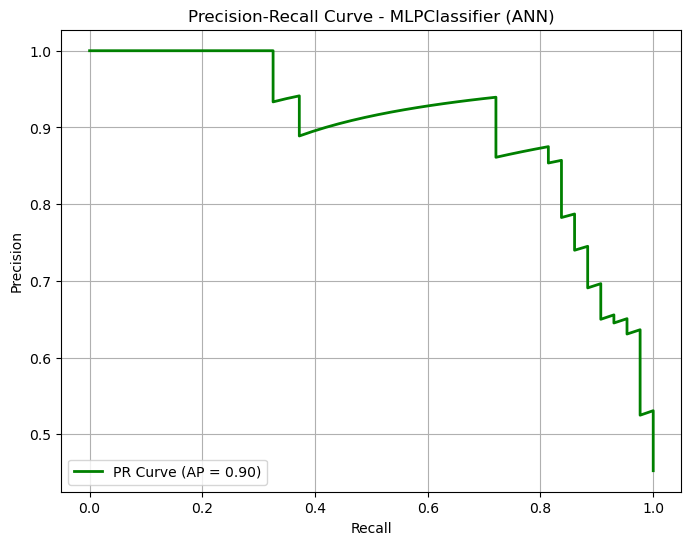
\includegraphics[width=0.35\textwidth]{prc-curve/ann.png} \\
\end{tabular}

\end{center}
    \caption{\textbf{PRC Curves of Different Classifiers}}
    \label{fig:prc-figure} 
\end{figure}

\section{Explainable AI }When AI is applied to real-life uses, it is essential to understand the AI itself. In this section, the aim was to determine how the machine learning model takes the decisions, based on what it predicts, what it predicts. Hence, LIME (Local Interpretable Model-Agnostic Explanation) was applied on the best performing model CatBoost to understand how the black box machine learning models operated the results\cite{ref14}. Fig.~\ref{fig:strongcase} and Fig.~\ref{fig:weakcase} illustrate the interpretation of the XAI in predicting 'Strong' and 'Weak' classes respectively, highlighting the contribution of individual features and their importance scores in the model’s decision-making process : \vspace{0.5cm}

\begin{figure}[H]
    \centering
    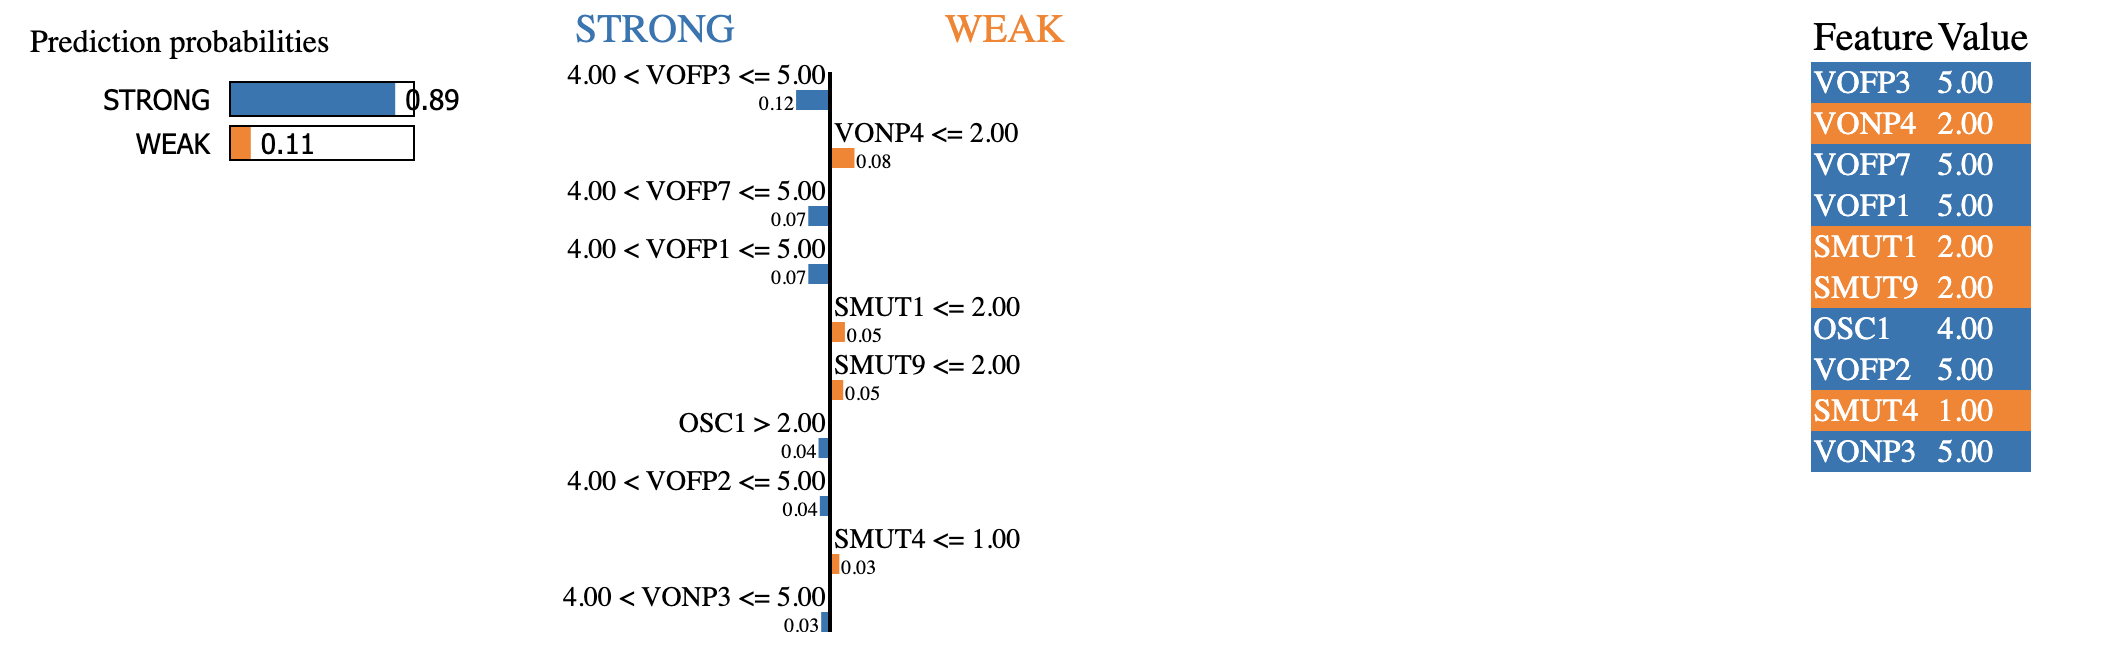
\includegraphics[width=13cm, height=5cm]{Project445/strong-LIME.png} % Replace with your image file
    \caption{\textbf{\small The Interpretation of Predicting The Strongly Partisan Case Using LIME}}
    \label{fig:strongcase}
\end{figure}

% First Figure
\begin{figure}[H]
    \centering
    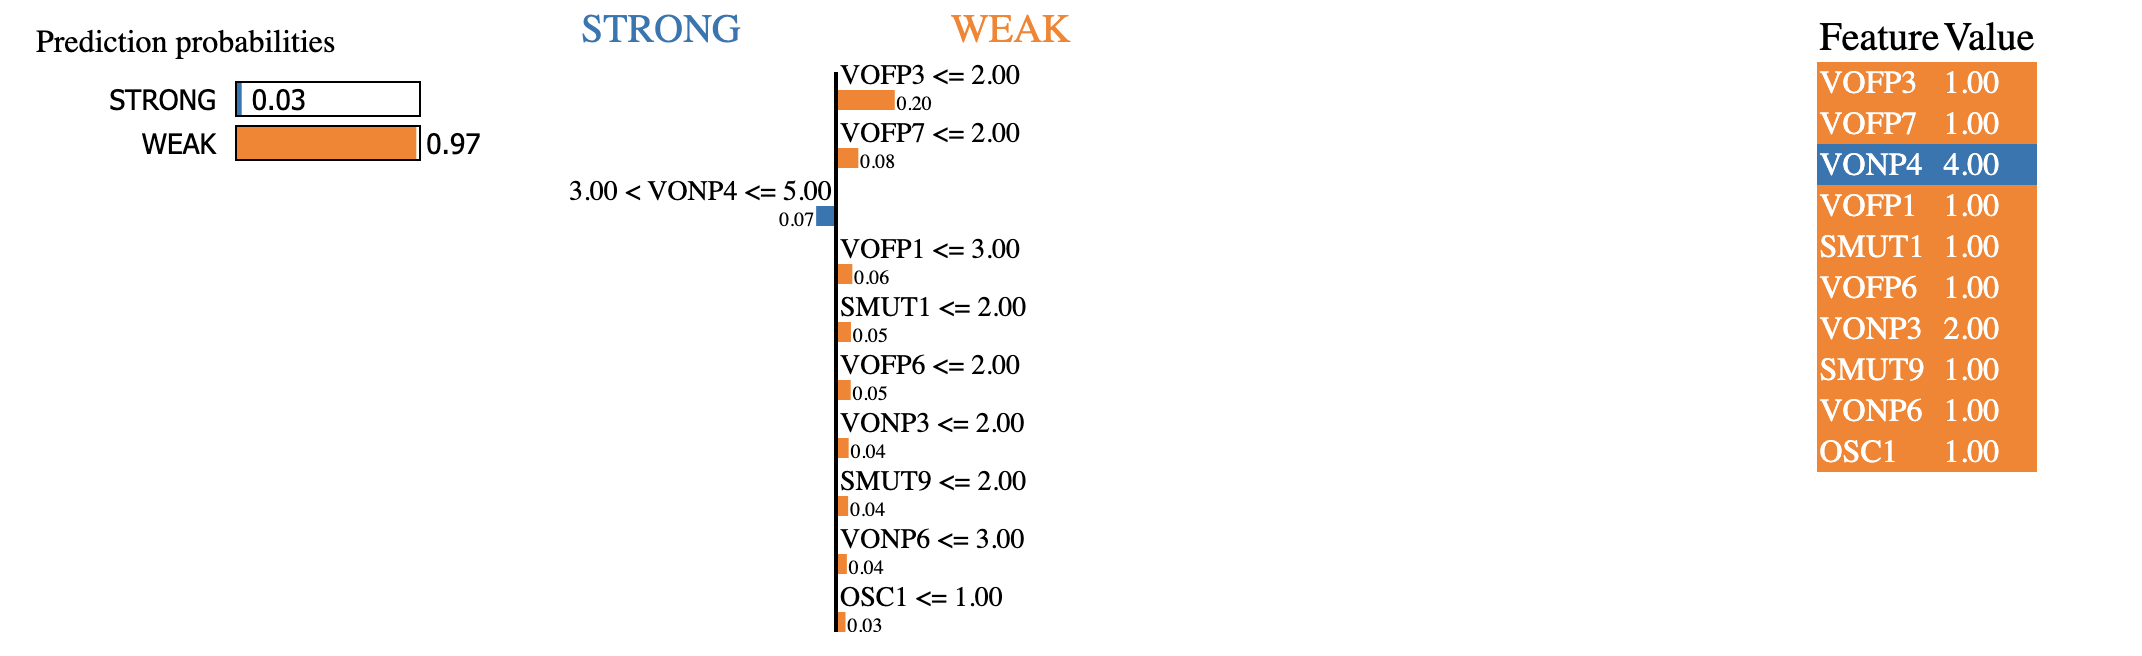
\includegraphics[width=13cm, height=5cm]{Project445/weak-LIME.png} % Replace with your image file
    \caption{\textbf{\small The Interpretation of Predicting The Weakly Partisan Case Using LIME}}
    \label{fig:weakcase}
\end{figure}

Fig.~\ref{fig:strongcase} shows that the CatBoost model predicts a strongly partisan case with 89\% confidence for the "Strong" class. Key features driving this decision include \texttt{4.00 $<$ VOFP3 $\leq$ 5.00}, \texttt{4.00 $<$ VOFP7 $\leq$ 5.00}, and \texttt{4.00 $<$ VOFP1 $\leq$ 5.00}, while \texttt{VONP4 $\leq$ 2.00} and \texttt{SMUT1 $\leq$ 2.00} contribute minimally to the "Weak" class.

 The statements represented by VOFP3, VOFP7, and VOFP1 are as follows:

	\begin{itemize}
    \item 	VOFP3: I participated in demonstrations or protests.
	\item 	VOFP7: I got involved in public interest groups, political action         groups, political clubs, or party committees.
	\item 	VOFP1: I volunteered for a campaign or other political cause.
    \item   VONP4: I forwarded a political e-mail or link to another person.
    \item   SMUT 1: I use social media to get information about current political events.
    \end{itemize}

    Fig.~\ref{fig:weakcase} highlights the weakly partisan case predicted with 97\% confidence for the "Weak" class. Dominant features include \texttt{VOFP3 $\leq$ 2.00}, \texttt{VOFP7 $\leq$ 2.00}, \texttt{VOFP1 $\leq$ 3.00}, and \texttt{SMUT1 $\leq$ 2.00}, while minor contributions from \texttt{3.00 $<$ VONP4 $\leq$ 5.00} support the "Strong" class.

\section{Manual Uniform Input Validation}
Alongside the assessment of the model through conventional performance metrics, we implemented a Manual Uniform Input Validation test. This step was implemented to evaluate the robustness and logical consistency of the model when subjected to extreme and uniform input cases. The rationale behind this validation approach was to understand how the model behaves when all responses in the input questionnaire are identical, representing extreme or neutral responses. This study also aimed to ensure that the model produces meaningful predictions under such conditions. The model is tested on the following hypothetical cases:

\begin{itemize}
    \item All responses are "Strongly Disagree":
   This scenario represents a negative sentiment across all questions. The objective here is to observe whether the model correctly identifies the weak partisanship.

\item All responses are "Disagree":
Similar to the first case but slightly less extreme, the prediction is weak, indicating minimal political involvement.

\item All responses are “Neutral”:
The model predicts strong partisanship, suggesting that neutral responses may reflect a default alignment for political engagement in the dataset.

\item All responses are “Agree”:
Based on this response the model prediction is strong, signifying a higher degree of political alignment or partisanship.

\item All responses are “Strongly Agree”:
Following the positive viewpoint in this response, the prediction remains strong, consistent with high levels of political agreement. 
\end{itemize}

This validation method is essential to understand how the model responds to extreme and balanced input scenarios. By testing uniform responses, we assess the model's ability to generalize beyond the complexity of real-world data and its reliance on specific response patterns. The results indicate that the model assigns weak partisanship to negative or disengaged responses, while neutral or positive responses trigger strong predictions. This validation serves to confirm the internal consistency and logical reasoning of the model, reinforcing confidence in its predictions. 


\section{Cross-Country Model Evaluation } Following the evaluation of the main model, an additional cross-country analysis is conducted to assess the adaptability and robustness of the predictive framework across different geographical and cultural contexts. This analysis aims to determine how well the model, trained on one country’s data, performs when tested on data from other countries. It is focused on demonstrating the model’s potential for application across different countries, provided that training data methods are carefully tailored. The overview of the cross-country workflow is demonstrated in Fig~\ref{fig:figure2}.\vspace{0.3cm}

	\subsection{Data Splitting Based on Country of Origin }
The dataset was divided into three country-specific subsets: the UK, Malaysia, and Pakistan. For each case:
	\begin{itemize}
	    \item The model is trained using the dataset from one specific country's data.
	    \item The trained model is then tested separately on the datasets of the other two countries, creating two distinct test scenarios.
	\end{itemize}

\subsection{Feature Selection for Each Country } Feature selection is conducted independently for each case to ensure the model is optimized for the training dataset. The same two-steps (Pearson's correlation and information gain algorithm) feature selection process applied in the main model is repeated for each country. 
\subsection{Rationale for Using the Best-Performing Model }The best-performing model, CatBoost from the main evaluation is chosen for this analysis due to its ability to handle the complexities of the dataset and provide consistent results. By leveraging this model, the cross-country evaluation focused on understanding the effects of training data diversity and country-specific features while maintaining a stable predictive framework.

\subsection{Results}
Table~\ref{tab:cross} provides a summary of the cross-country model's performance measures. The model is applied through CatBoost classifier achieving an accuracy of 0.87 when tested on Malaysia and trained on the UK dataset. Its' F1 scores of 0.85 (Strong) and 0.89 (Weak) show balanced performance. With an accuracy of 0.78, the model's performance slightly declines when tested on Pakistan after being trained on the UK dataset. The corresponding F1 scores are 0.83 (Strong) and 0.71 (Weak).
The Malaysia-to-UK combination has an accuracy of 0.78 while F1 scores are 0.85 (Strong) and 0.57 (weak). The model achieves an accuracy of 0.76 when evaluated on Pakistan and F1 score of 0.82 and 0.65 for "Strong" and "Weak" classes respectively.
With an accuracy of 0.79, the model that was trained on Pakistan and tested on the UK has F1 score of 0.49 for "Weak" class, whereas the "Strong" class receives an F1 score of 0.87.
Lastly, the model gets the best accuracy of 0.89 among all configurations when evaluated on Malaysia after being trained on Pakistan having the highest F1 scores of 0.87 (Strong) and 0.91 (Weak). \vspace{0.5cm}

\begin{table}[H]
\centering
\begin{tabular}{|c|c|c|cc|cc|cc|}
\hline
\textbf{Train Set} & \textbf{Test Set} & \textbf{Accuracy} & \multicolumn{2}{c|}{\textbf{Precision}} & \multicolumn{2}{c|}{\textbf{Recall}} & \multicolumn{2}{c|}{\textbf{F1 Score}} \\ \cline{4-9} 
                   &                   &                   & \textbf{Strong}    & \textbf{Weak}    & \textbf{Strong}   & \textbf{Weak}   & \textbf{Strong}      & \textbf{Weak}     \\ \hline
UK          & Malaysia         & 0.87              & 0.81               & 0.92             & 0.81              & 0.87           & 0.85                & 0.89              \\ \hline
UK         & Pakistan         & 0.78              & 0.88               & 0.65             & 0.78              & 0.79           & 0.83                & 0.71              \\ \hline
Malaysia         & UK        & 0.78              & 0.81               & 0.68             & 0.9              & 0.49            & 0.85                & 0.57              \\ \hline
Malaysia          & Pakistan       & 0.76              & 0.82               & 0.65            & 0.82              & 0.65            & 0.82                & 0.65              \\ \hline
Pakistan         & UK         & 0.79              & 0.78               & 0.89             & 0.98              & 0.34            & 0.87                & 0.49              \\ \hline
Pakistan         & Malaysia        & 0.89              & 0.82               & 0.95             & 0.94              & 0.87            & 0.87                & 0.91              \\ \hline
\end{tabular}
\caption{Performance Metrics for the Cross-Country Model}
\label{tab:cross}
\end{table}

% Discussion
\section{Discussion}
This study aimed to analyse political partisanship by machine learning models using survey data. The conducted research took responses from three countries and amounted to a total sample of 472. Despite the subjective complexities of people’s political orientation, we were able achieve a noteworthy performance[result].  The uniqueness of this data[dataset link] stems from the fact that the survey was based on the Motive-Incentive-Activation-Behavior (MIAB) model\cite{ref5}.  This framework helps to understand the motivations behind a respondent’s political behavior. The survey aids in identifying the key incentives which could be both online and offline behavior that may underline partisanship. This investigation produced results shown in Fig.~\ref{fig:strongcase} and Fig.~\ref{fig:weakcase} imply that, while online engagement is impactful, it may not yet fully replace the role of traditional political involvement in predicting partisan behavior. Individuals who actively participate in demonstrations or protests are prone to having stronger partisanship, additionally involvement in political group or committees are key factors. Moreover, the respondents who take information from social media to learn about political events often have high political bias. Hence offline activities remain crucial touchpoint for mobilization, but the influence of online platforms should not be underestimated, particularly as digital adoption continues to rise globally. 


\section{Limitation}

Using machine learning to predict political affiliation from poll datasets can be difficult for a number of reasons. When people fill out surveys, especially about political issues, the answers are subjective and can be affected by biases like social desirability or acquiescence bias, which means people may give answers they think are expected. The qualitative nature of survey data, which frequently includes capturing complex human behavior that cannot be fully quantified, presents additional challenges for machine learning models. Although Explainable AI techniques help interpret results, they may not fully address the complexities of human decision-making. These limitations emphasize the need for caution when interpreting results and suggest that combining machine learning with qualitative approaches can provide a more holistic understanding of political partisanship.


\section{Conclusion}

This research synthesizes the need for understanding political favoritism among people through the lens of Artificial Intelligence. By incorporating machine learning approach, actionable insights are produced. The findings underscore the enduring importance of offline activities, such as participation in protests and political campaigns, while highlighting the complementary role of online platforms in shaping political behavior. The best-performing model, CatBoost, achieved an accuracy of 87\% and provided interpretable results through explainable AI techniques. These insights revealed that offline activities dominate as predictors of partisanship, but online engagement is increasingly significant. Additionally, the The cross-country model validates the transferability of the model. Despite these achievements, challenges such as the qualitative nature of survey responses, cultural variability, and biases in self-reported data limit the of the results. In future, this research can be explored by using advanced techniques like deep learning that would utilize complex data types like images or videos, to uncover richer insights into political partisanship. There’s also potential to transform this work into a practical tool, like a software application or web platform, that policymakers could use to gain real-time insights and make decisions. Collecting larger and more diverse datasets would further improve the model’s reliability across different populations. Collaborating with experts in political science or sociology could also provide valuable perspectives, adding depth to the understanding of human behaviors behind political partisanship. These future advancements could make the model not just a research tool but a powerful resource for handling political challenges on a larger scale.
 
% References
\begin{thebibliography}{9}
\small \bibitem{ref1}\label{ref1}
\textit{Divided we stand: The rise of political animosity},
Available: \url{https://tinyurl.com/ykkx5nc2}.

\small \bibitem{ref2}\label{ref2}
\textit{The Rise of Partisan Affective Polarization in the British Public},
Available: \url{http://dx.doi.org/10.2139/ssrn.3477404}.

\small
\bibitem{ref3}\label{ref3}
\textit{Causes of Political Polarization in Pakistan},
Available: \url{https://tinyurl.com/5n7yt42v}. 

\bibitem{ref4}\label{ref4}
 \textit{Survey data to unveil the power of political crowdsourcing on social media},
Available: \url{https://doi.org/10.1016/j.dib.2024.110758}.

\bibitem{ref5}\label{ref5}
\textit{A Methodological Framework for Crowdsourcing in Research},
Available: \url{https://tinyurl.com/mvznbynt}.

\bibitem{ref6}\label{ref6}
\textit{How are Online and Offline Political Activities Connected?
A Comparison of Studies},
Available: \url{https://tinyurl.com/58a6r3ap}.

\bibitem{ref7}\label{ref7}
\textit{Hong, Y. and Lin, T. (2017) The Impacts of Political Socialization on People’s Online and Offline Political Participation—Taking the Youth of Singapore as an Example. Advances in Journalism and Communication,},
Available: \url{https://doi.org/10.4236/ajc.2017.51003}.

\bibitem{ref8}\label{ref8}
\textit{A Machine Learning Pipeline to Examine Political Bias with Congressional Speeches},
Available: \url{https://tinyurl.com/2farnmuw}.

\bibitem{ref9}\label{ref9}
\textit{The slacktivism crossroad: causal relationships between online and offline political participation},
Available: \url{https://api.semanticscholar.org/CorpusID:238864473}.

\bibitem{ref10}\label{ref10}
\textit{Modeling Political Orientation of Social Media Posts: An Extended Analysis},
Available: \url{https://tinyurl.com/2sbu7jr3}.

\bibitem{ref11}\label{ref11}
\textit{Confusion Matrix},
Available: \url{https://tinyurl.com/47a6467y}.

\bibitem{ref12}\label{ref12}
\textit{The receiver operating characteristic (ROC) curve},
Available: \url{https://tinyurl.com/4skw3rb6}.

\bibitem{ref13}\label{ref13}
\textit{Precision-Recall-Gain Curves:
PR Analysis Done Right},
Available: \url{https://tinyurl.com/3v5snhts}.

\bibitem{ref14}\label{ref14}
\textit{"Why Should I Trust You?": Explaining the Predictions of Any Classifier},
Available: \url{https://arxiv.org/abs/1602.04938v3}.

\bibitem{ref15}\label{ref15}
\textit{"Using Machine Learning to Measure Political Polarization on Social Media},
Available: \url{https://tinyurl.com/39mrezas}.

\end{thebibliography}
\end{document}

